\documentclass{ieeeaccess}
\usepackage[utf8]{inputenc}
\usepackage{amsmath,amssymb,amsthm}
\usepackage{graphicx}
\usepackage{multirow}
\usepackage{cite}
\usepackage{textcomp}
\usepackage{array}
\usepackage{algorithm}
\usepackage{algpseudocode}
\usepackage{url}
\usepackage{listings}

\lstdefinelanguage{drgl}{
  morekeywords={RETAIN,DELETE,HOLD,MUST_DELETE,ALLOW_DELETION,RECORDS,WHERE,FOR,AFTER,IN,BECAUSE,MATTER,PROPAGATE,VIA,UNTIL,RELEASED,UNLESS,AND,OR,IN,CONTAINS,BETWEEN,CREATION,LAST_MODIFIED,LAST_ACCESSED,EVENT,END_OF_FISCAL_YEAR,DURATION_OF,PERMANENT,DAYS,MONTHS,YEARS,SELECT,EXPLAIN,STATUS,AT,COUNT,FROM},
  sensitive=true,
  morecomment=[l]{--},
  morestring=[b]'
}
\lstset{
  basicstyle=\ttfamily\small,
  keywordstyle=\bfseries,
  commentstyle=\itshape,
  stringstyle=\itshape,
  breaklines=true,
  showstringspaces=false,
  frame=single,
  columns=fullflexible
}

\newtheorem{proposition}{Proposition}
\newtheorem{corollary}{Corollary}
\newtheorem{definition}{Definition}

\title{T-RKG and DRGL: A Knowledge-Based System and Declarative Language for Cross-System Regulatory Conflict Detection and LLM-Assisted Policy Compilation in Enterprise Records Governance}

\author{\uppercase{Kishore Pulagam}\authorrefmark{1}\orcid{0009-0006-7929-8699}}

\address[1]{Northwestern University, Evanston, IL, USA and PayPal Data Services}
\date{2026-05-25}

\doi{10.1109/ACCESS.2026.XXXXXXX}

\begin{document}

\maketitle

\begin{abstract}
Enterprise records governance is a distributed coordination problem. Document retention schedules, legal hold obligations, multi-jurisdictional compliance requirements, and natural-language regulatory policies are enforced by systems that share no unified regulatory knowledge and no common machine-readable policy substrate. Three structural gaps follow. First, conflicts between regulations applicable to the same record are invisible to siloed enforcement: a single payment transaction can carry tax retention obligations from one jurisdiction, privacy erasure obligations from another, and audit obligations from a third, with each obligation conditioning on a different attribute that lives in a different source system. Second, governance rules are expressed either as native platform configurations or as ad-hoc scripts, with no formal language able to encode retention, hold, and deletion semantics with the temporal precision the regulations require. Third, translating natural-language regulations into executable rules is manual, slow, and error-prone, while direct application of large language models is unsafe because LLM outputs lack the formal guarantees regulators expect. This paper presents an integrated knowledge-based system addressing all three gaps. T-RKG (Temporal Records Knowledge Graph) is a formal governance ontology of 47 classes and 23 object properties encoding records as composite governance entities, with a typed temporal relationship model that governs hold propagation through declared edge semantics, and a conflict-detection mechanism that applies ontological applicability reasoning. DRGL (Declarative Records Governance Language) is a domain-specific language with formal semantics over the T-RKG model, supporting five rule families (RETAIN, DELETE, HOLD, MUST\_DELETE, ALLOW\_DELETION) with temporal triggers, jurisdiction qualifiers, and configurable propagation. An LLM-assisted compilation pipeline translates natural-language regulatory text into DRGL with three-stage symbolic validation (syntax, type, conflict) that catches and recovers compiler errors before deployment. Evaluated across five random seeds at six dataset scales (1{,}000 to 100{,}000 records), T-RKG detects 55 to 4{,}672 regulatory conflicts per dataset, of which 4 to 831 are cross-domain conflicts that two structurally siloed baselines cannot detect (Corollary~1). T-RKG attains F1 of $0.823 \pm 0.011$ under 10\% per-attribute label noise. On a corpus of 50 real-world regulatory policies, the LLM-assisted DRGL compilation pipeline achieves 95\% functional equivalence with expert-authored ground truth (versus 44\% for zero-shot GPT-4 and 66\% for few-shot baselines), with symbolic validation detecting 100\% of syntax/type/temporal/reference errors and 92\% of subtle rule conflicts. End-to-end governance accuracy on a 10{,}000-record repository reaches 96\% F1.
\end{abstract}

\begin{keywords}
Knowledge-based systems, knowledge graph, ontology, regulatory compliance, temporal reasoning, decision support, records governance, domain-specific language, large language models, neuro-symbolic AI
\end{keywords}

\section{Introduction}

Consider what happens when a litigation hold is issued against a custodian whose email resides on one platform, whose working documents live in a separate document management system, and whose contracts are stored in a third system. The hold is placed. The email system preserves the custodian's messages. The attachments to those messages remain in the document management system. They are unaffected. That system has received no instruction and possesses no knowledge of the hold. The relationship between an email and its attachment is obvious to any human reviewer. It has no formal representation in the technical infrastructure. It cannot be reasoned over because it has never been encoded.

This is not an edge case. Industry survey data~\cite{sedona2019} suggest that 60\% to 80\% of documents eventually identified as relevant in litigation are surfaced through relational links rather than direct custodian identification. The hold methodology that ignores cross-system relationships is incomplete by design.

Regulatory fragmentation compounds the structural problem. A financial services organization that handles personal data for European customers may find that the same record is simultaneously governed by GDPR Article~17, which requires deletion upon a verified erasure request, and by SOX Section~802, which mandates a seven-year retention period for certain financial records. Neither the privacy platform enforcing GDPR nor the compliance platform enforcing SOX holds a complete picture. The privacy platform typically lacks the metadata needed to determine SOX applicability. The compliance platform lacks the PII classification that would trigger GDPR obligations. The conflict is real. It is also invisible to any system that cannot reason across both regulatory contexts simultaneously~\cite{edrm,iso15489,zubulake}.

A third observation motivates the work. Commercial records governance products in this space (Microsoft Purview, OpenText, IBM FileNet, Veritas, OneTrust, and similar vendors) treat the unit of governance as a content object that arrives in a managed repository. That framing was adequate when most regulated information was filed-style content (memos, statements, reports). It is no longer adequate. A regulated record in a modern enterprise is often a composite. A single payment transaction might carry tax-retention obligations from the IRS, privacy-erasure obligations from GDPR for the European data subject, audit obligations from SOX for the public-company parent, and SEC retention obligations on the trade leg. Each obligation conditions on a different attribute. The PII flag that triggers GDPR lives in the customer-data system. The public-company flag that triggers SOX lives in organizational metadata. The transaction record itself lives in the ERP. The geographic attribute that triggers HGB for a German subsidiary may live in a separate compliance system. A governance architecture that only sees content cannot detect any of this. The conflict exists in the conjunction of attributes spread across systems.

A fourth gap is the policy-language gap. Even granted a unified knowledge layer over records and regulations, the rules themselves originate in natural-language statutes, regulator guidance documents, and corporate retention schedules. Translating that text into executable governance rules is currently a manual exercise in legal-technical bilingualism. The result is either expert-authored configuration deep inside commercial products (auditable only by re-reading the configuration) or ad-hoc scripts (auditable only by re-reading the code). Neither is a policy language in the sense the regulatory-knowledge-representation literature uses the term~\cite{xacml,rego,cedar,legalruleml}. Recent work has explored large language models as a translation layer from natural-language policy to formal rules~\cite{nl2ltl,req2ltl,nist_lawal2025}, but LLMs alone cannot be trusted to produce compliance-grade rules: they hallucinate, they invent attributes that do not exist in the target schema, and they cannot self-detect conflicts with previously authored rules. The neuro-symbolic literature~\cite{garcez2020,bifrostrag} establishes that LLM outputs must be paired with symbolic verification before they can be used in any setting where errors carry legal consequences.

What all four cases require is an integrated layer that (a) unifies records and regulations as a queryable knowledge graph, (b) expresses governance policies in a formal language with temporal semantics, and (c) compiles natural-language regulations into that language with symbolic guarantees. Better engineering within existing silos does not provide this. The silos themselves are the problem; the absence of a formal policy substrate is the second problem; and the absence of a verified translation pipeline is the third.

\subsection{Contributions}

This paper presents an integrated knowledge-based system addressing all four gaps. The contributions are as follows.

\begin{enumerate}
    \item A formal governance ontology comprising 47 classes (across five modules: Record, Actor, Governance, Regulatory, Conflict) and 23 object properties, plus six reified temporal-relationship subclasses. The ontology encodes records as composite governance entities that aggregate content, transactional, geographic, custodial, and organizational attributes. It is delivered in OWL/Turtle as supplementary material.
    \item A typed temporal relationship model in which hold propagation is governed by the declared semantic properties of each relationship type. Attachment relationships propagate holds by default. Passing references do not. Defaults are overridable per legal matter, enabling configurable, auditable propagation policies.
    \item A conflict detection mechanism that applies ontological applicability reasoning. The reasoner determines which regulations govern a given record and whether those regulations impose contradictory requirements. The mechanism requires unified regulatory knowledge.
    \item DRGL (Declarative Records Governance Language): a domain-specific language with formal semantics over the T-RKG model, supporting five rule families (RETAIN, DELETE, HOLD, MUST\_DELETE, ALLOW\_DELETION) with temporal triggers, jurisdictional qualifiers, propagation specifications, and rationale citations. DRGL grammar is specified in Extended Backus--Naur Form; semantics are defined as a function from time to per-record governance state.
    \item An LLM-assisted DRGL compilation pipeline. Natural-language regulatory policies are translated to DRGL through an LLM augmented with the formal grammar, the target schema, and few-shot examples; the output passes through a three-stage symbolic validator (syntax, type, semantic-conflict) with an error-feedback loop that recovers most invalid generations within one to two retries.
    \item Empirical evaluation across two strands. (a)~T-RKG conflict detection across five random seeds and six dataset sizes (1K to 100K records). T-RKG detects 55 to 4{,}672 conflicts per dataset, of which 4 to 831 are cross-domain. Both baselines detect zero cross-domain conflicts at every scale, an outcome formalized as Corollary~1. Per-record applicability F1 against an independently-constructed reference is reported in clean and noised regimes; under 10\% input label noise T-RKG attains $0.823 \pm 0.011$. (b)~DRGL compilation on a corpus of 50 real-world regulatory policies. The integrated pipeline achieves 95\% functional equivalence with expert-authored ground truth versus 44\% for zero-shot GPT-4 and 64--66\% for few-shot LLM baselines. Symbolic validation detects 100\% of syntax/type/temporal/reference errors and 92\% of subtle rule conflicts. End-to-end governance accuracy on a 10{,}000-record repository reaches 96\% F1 across retention, hold, and disposition scenarios.
\end{enumerate}

\section{Related Work}

\subsection{Knowledge-Based Systems for Legal and Regulatory Compliance}

Formal knowledge representation for legal reasoning has a documented history. It extends back at least to Sergot et al.~\cite{sergot1986}, whose encoding of the British Nationality Act as a Prolog logic program demonstrated that statutory rules could in principle support automated query answering. Ashley~\cite{ashley2017} surveys AI approaches to legal analytics, observing that knowledge representation remains the central unsolved challenge when the goal is to capture the interactions among rules, precedents, and contextual conditions that determine applicability. LegalRuleML~\cite{legalruleml} addresses part of this through an XML vocabulary for defeasible legal norms. LKIF Core~\cite{lkif} provides a legal knowledge interchange format supporting cross-system reasoning. Akoma Ntoso~\cite{akomantoso} is the OASIS-standard XML vocabulary for legislative documents, against which EUR-Lex publishes; T-RKG profiles regulations as encoded \texttt{RegulationProfile} objects rather than parsing Akoma-Ntoso source, and an automated ingestion path from Akoma-Ntoso XML is roadmap work.

In financial compliance specifically, knowledge-based approaches have been applied to anti-money laundering and KYC processes~\cite{weber2019}. FIBO~\cite{fibo} standardizes financial concepts for regulatory reporting. RegTech draws on computational methods including NLP over raw regulatory text to support compliance verification~\cite{arner2017,legalbert}. Defeasible deontic logic~\cite{governatori2013} provides the formal framework for resolving conflicts between obligations and permissions by lex-superior, lex-specialis, and lex-posterior precedence; T-RKG's Priority conflict family duplicates this resolution structure in tabular form, and §V-C describes the bridge.

\subsection{Enterprise Knowledge Graphs and Records Governance Products}

The practical deployment of knowledge graphs in enterprise settings is well documented. Galkin et al.~\cite{galkin2017} establish that graph-based data integration enables analytical capabilities that siloed relational architectures cannot support. Noy et al.~\cite{noy2019} report on deployments at Google, Microsoft, and several major financial institutions. Pan et al.~\cite{pan2024} survey the more recent trajectory toward integrating large language models with knowledge graphs. Hogan et al.~\cite{hogan2021} is the canonical KG survey of the post-2018 period. Bizer et al.~\cite{bizer2009,linkeddata} frame the broader Linked Data context. KG.GOV~\cite{kggov2025} is the closest analog to T-RKG's framing, positioning knowledge graphs as governance infrastructure for AI workflows; the work T-RKG presents is narrower, targeting cross-regulation conflict detection in records governance specifically rather than AI-workflow governance writ large.

Commercial records governance products are a different class. They include Microsoft Purview~\cite{purview}, OpenText InfoArchive, IBM FileNet Records Manager, Veritas Enterprise Vault, OneTrust, and Smarsh. These products treat the unit of governance as a content object: an email body, a document file, a chat message. Retention rules attach to content objects by file type, by container, or by classification tag. This framing is correct for the historical use case (statements, memos, reports) and remains adequate where the regulated quantity is the content itself.

The framing is inadequate when the regulated quantity is a composite of attributes spread across systems. A payment-transaction record subject to GDPR-erasure obligations on one attribute and SOX-retention obligations on another cannot be represented faithfully as a single content object. The content of the transaction is a row in the ERP. The PII attribute resides in the customer-data system. The public-company attribute resides in organizational metadata. T-RKG treats the record as a composite governance entity that aggregates these attributes through the ontology, then runs applicability reasoning over the aggregate. Section~\ref{sec:composite} formalizes this distinction.

\subsection{Policy Languages and Access Control}

Formal languages for policy specification have been studied extensively in access control. XACML~\cite{xacml} provides an XML-based standard for expressing access policies; Cedar~\cite{cedar} and Rego~\cite{rego} are more recent attribute-based and policy-as-code formulations targeting cloud authorization. NGAC~\cite{ngac} offers a flexible attribute-based access-control model with formal semantics. ODRL~\cite{odrl} is the W3C Recommendation for permissions, prohibitions, and obligations over digital assets. All of these languages target access decisions (permit/deny) and lifecycle management for entitlements; none natively encodes retention-period semantics, legal-hold propagation across typed relationships, or jurisdiction-conditioned deletion mandates, which are the operative concerns of records governance. DRGL fills this gap; §IV-A formalizes the design principles that distinguish it from XACML and Cedar specifically.

\subsection{LLMs for Code and Specification Generation}

Large language models have demonstrated capability in code generation~\cite{codex} and program synthesis~\cite{austin2021}. Recent work translates natural language into formal specifications: NL2LTL~\cite{nl2ltl} for linear temporal logic, Req2LTL~\cite{req2ltl} for requirements engineering, NIST's investigation of LLM-based access-control policy translation~\cite{nist_lawal2025}. The general lesson is that LLM-only translation is brittle (hallucination, schema drift, conflict-blindness); pairing the LLM with a symbolic validator and an error-feedback loop is the established mitigation. Garcez et al.~\cite{garcez2020} survey the neuro-symbolic paradigm; BifrostRAG~\cite{bifrostrag} applies it to regulatory compliance question answering. The DRGL compilation pipeline in §V follows this neuro-symbolic architecture: LLM for semantic interpretation, symbolic validator for correctness guarantees.

\subsection{Temporal Knowledge Graph Reasoning}

The formal treatment of time in knowledge graphs was established by Gutierrez et al.~\cite{gutierrez2007}, who introduced validity intervals on RDF triples. Allen's interval algebra~\cite{allen1983} provides the formal machinery for reasoning about temporal relationships between intervals. The temporal-database foundations of valid-time and transaction-time separation were codified by Snodgrass and collaborators~\cite{snodgrass1995,jensen1997}. Contemporary temporal KG research is oriented primarily toward link prediction; representative methods include TransE~\cite{transe}, RotatE~\cite{rotate}, TimePlex~\cite{timeplex}, TLogic~\cite{tlogic}, TeMP~\cite{temp}, and TIE~\cite{tie}, as surveyed in Cai et al.~\cite{cai2023}. T-RKG's temporal requirements fall in the interval-based, point-in-time query-answering category rather than the completion category; §V-E describes the bitemporal modeling that supports historical reconstruction.

\subsection{Ontology Engineering for Decision Support}

Gruber~\cite{gruber1995} formalized an ontology as a specification of a conceptualization. Guarino et al.~\cite{guarino2009} sharpen the ontological distinctions relevant to knowledge sharing. Uschold et al.~\cite{uschold1998} demonstrate the Enterprise Ontology's utility for business reasoning. Gr\"{u}ninger and Fox~\cite{gruninger1995} introduced the competency question methodology. The T-RKG competency questions are listed in Section~\ref{sec:cqs} and each is paired with a passing test in the supplementary code. Domain-specific ontologies for decision support have been developed in healthcare~\cite{schriml2019}, finance~\cite{fibo}, and industrial automation~\cite{ringsquandl2015}. Brank et al.~\cite{brank2005} survey ontology evaluation methodology. SHACL~\cite{shacl} provides the W3C constraint language for RDF graphs; the relationship-class constraints (\texttt{propagatesHold}, \texttt{strengthLevel}) in §IV-C are equivalent in expressivity to SHACL property shapes and could be migrated.

\subsection{Evaluation Data and Access Constraints}

Access to real enterprise records data presents evaluation challenges that are structural rather than incidental. Legal privilege, privacy regulation, and contractual confidentiality agreements create barriers that do not yield to the standard remedy of collecting a large labeled dataset and splitting it for evaluation. For such settings, synthetic generation with parameterized distributions has been established as a methodologically sound alternative. Hubert et al.~\cite{pygraft} demonstrate configurable synthetic schema and KG generation. Van der Aalst~\cite{vanderaalst2016} examines evaluation methodology for process mining, a domain facing nearly identical data access constraints. T-RKG's evaluation follows this practice. The synthetic generator is parameterized against industry-reported data distributions~\cite{databerg,igrm}. To bound the limitation that synthetic data carries for production claims, Section~\ref{sec:robustness} reports a parameter-sweep robustness experiment showing that T-RKG behavior varies smoothly with the two parameters most likely to differ across organizations.

\section{Preliminaries}

\subsection{Core Concepts}

\textit{Record.} A record $r \in R$ is an information object subject to governance, characterized by type $\tau(r) \in T$, creation time $t_c(r)$, custodian $\kappa(r) \in C$, source system $\sigma(r) \in S$, jurisdiction $\zeta(r) \in J$, and an attribute set $a(r)$ including PII and PHI indicators.

\textit{Temporal Relationship.} A temporal relationship between records $r_i, r_j \in R$ is a tuple $(r_i, r_j, \rho, [t_s, t_e])$ where $\rho \in P$ denotes the relationship type and $[t_s, t_e]$ is the validity interval.

\textit{Legal Hold.} A legal hold $h = (m, S, P', [t_s, t_e])$ associated with matter $m \in M$ preserves all records matching scope predicate $S$, propagates transitively through relationship types $P' \subseteq P$, and remains active during $[t_s, t_e]$.

\textit{Regulatory Conflict.} A regulatory conflict exists for record $r$ when at least two regulations $\gamma_1, \gamma_2 \in \Gamma$ are simultaneously applicable to $r$ and their operative requirements are mutually exclusive over a shared temporal applicability window.

\subsection{Problem Statement}

Given a set of enterprise records $R$ distributed across source systems $S$, inter-record temporal relationships $E$, a set of applicable regulatory frameworks $\Gamma$, and a set of active legal matters $M$, the enterprise records governance problem requires five capabilities: (1)~knowledge unification across heterogeneous source systems; (2)~hold propagation through inference over typed relationship semantics; (3)~conflict detection via ontological applicability reasoning; (4)~temporal query answering at arbitrary historical or current time points; and (5)~a formal policy language able to express retention, hold, and deletion rules in a form regulators can audit and engineers can execute.

\subsection{The Composite-Record Model}
\label{sec:composite}

A standard records-management view treats a record as a content object with metadata. Formally, that view is a pair $(c, m)$ where $c$ is the content (a file, an email body, a chat message) and $m$ is a set of metadata key-value pairs attached to $c$. Retention and deletion rules attach to $(c, m)$ through type, classification, or container.

T-RKG generalizes the record to a composite entity. A T-RKG record is the tuple $(c, A, \sigma, \kappa, \zeta)$ where $c$ is content as before, $A$ is an attribute multimap over a fixed schema (PII, PHI, public-company status, customer identifier, transaction identifier, etc.), $\sigma$ is the source system of record, $\kappa$ is the custodian, and $\zeta$ is the jurisdiction. Individual attributes in $A$ may originate from different source systems and be aggregated under $r$'s identity. Regulatory applicability is a predicate over $A$, not over $c$. Formally, for a regulation $\gamma$ with applicability profile $\phi_\gamma$:
\begin{equation}
    \mathrm{applicable}(r, \gamma) \iff \phi_\gamma(\tau(r), \zeta(r), A(r), m_{\mathrm{org}})
\end{equation}
where $m_{\mathrm{org}}$ are organizational metadata that do not vary per record.

This generalization is the substantive distinction from commercial governance products discussed in Section~II-B. Where those products evaluate retention rules over $(c, m)$, T-RKG evaluates over the broader attribute set $A$ that may live across source systems. The cross-domain conflicts the evaluation in Section~\ref{sec:rq1} reports are conflicts that are visible only in the composite view. The conjunction of (PII flag, public-company flag, jurisdiction) that triggers them does not exist in any single source system.

\section{The T-RKG Ontology}

\subsection{Overview}

Forty-seven classes, distributed across five modules, form the T-RKG ontological structure: Record (12 classes), Actor (6), Governance (12), Regulatory (10), Conflict (7). A separate Temporal Relationship sub-module reifies six relationship subclasses whose semantic properties drive propagation. Twenty-three object properties and 34 data properties complete the relational structure. The full ontology is provided as \texttt{ontology/trkg.ttl} in the supplementary material. Axioms remain within OWL~2~RL~\cite{owl2}, permitting forward-chaining materialization with a fixed-point semantics that the conflict-detection algorithm assumes.

\subsection{Record Module}

Twelve record classes are organized as a subclass hierarchy: \texttt{Record} with subclasses \texttt{Email}, \texttt{Document} (with \texttt{MedicalRecord}, \texttt{Spreadsheet}), \texttt{Chat}, \texttt{Ticket}, \texttt{Contract}, and \texttt{FinancialRecord} (with \texttt{AuditWorkpaper}, \texttt{Invoice}, \texttt{TaxRecord}). Type granularity matters for applicability reasoning. SOX Section~802 applies to \texttt{AuditWorkpaper} and \texttt{FinancialRecord} but not to \texttt{Chat}. GDPR Article~17 applies conditionally to any type carrying a PII flag. Each record instance is connected to its source system via \texttt{managedBy}, to its custodian via \texttt{hasCustodian}, and to its current governance state via \texttt{hasGovernanceState}.

\subsection{Temporal Relationship Module}

Inter-record relationships are represented as reified typed classes rather than as bare edges. Seven concrete subclasses are defined: \texttt{AttachmentRelationship}, \texttt{ThreadRelationship}, \texttt{DerivationRelationship}, \texttt{ReferenceRelationship}, \texttt{DuplicateRelationship}, \texttt{ContainerRelationship}, and \texttt{VersionRelationship}. Two properties on each relationship class are queried during propagation: \texttt{propagatesHold} (Boolean) and \texttt{strengthLevel} (ordinal). Attachment relationships, expressing content dependency, carry $\texttt{propagatesHold} = \mathrm{true}$ by default. Reference relationships default to false. All defaults are overridable at the matter level. Constraints of this form are equivalently expressible as SHACL property shapes~\cite{shacl}; T-RKG embeds them in the ontology for closer coupling with the rule layer.

\subsection{Regulatory Module}

Nine regulatory frameworks are encoded as subclasses of \texttt{Regulation}: \texttt{DataProtectionRegulation} (GDPR, CPRA, PIPEDA), \texttt{FinancialRegulation} (SOX, SEC, FINRA), \texttt{HealthRegulation} (HIPAA), \texttt{TaxRegulation} (IRS), and \texttt{NationalCommercialLaw} (HGB). Each regulation instance links to applicable jurisdictions through a hierarchical structure in which $\mathrm{subJurisdiction}$ is declared \texttt{owl:TransitiveProperty} so that the assertion $\mathrm{US} \supset \mathrm{US\text{-}CA}$ and $\mathrm{EU} \supset \mathrm{EU\text{-}DE}, \mathrm{EU\text{-}FR}$ allows applicability to be inherited downward from parent to child jurisdiction.

\subsection{Conflict Module and Inference Axioms}

Four conflict types are represented: RetentionDeletion, Jurisdiction, HoldDeletion, and Priority. A fifth (Procedural) is defined and instantiated with one rule (GDPR Art.~33 vs.\ SEC Reg-S-K Item 1.05) but not yet exercised in the empirical evaluation. Three inference axioms connect these types to record instances:
\begin{align}
&\mathrm{subjectTo}(r, \gamma) \leftarrow \mathrm{inJurisdiction}(r, j) \nonumber \\
&\quad \wedge\ \mathrm{appliesIn}(\gamma, j') \wedge \mathrm{subJurisdiction}(j, j') \tag{Ax.~1}
\end{align}
\begin{align}
&\mathrm{hasConflict}(r, c) \leftarrow \mathrm{subjectTo}(r, \gamma_1) \nonumber \\
&\quad \wedge\ \mathrm{subjectTo}(r, \gamma_2) \wedge \mathrm{conflictType}(\gamma_1, \gamma_2, c) \tag{Ax.~2}
\end{align}
\begin{align}
&\mathrm{underHold}(r_2, h) \leftarrow \mathrm{underHold}(r_1, h) \nonumber \\
&\quad \wedge\ \mathrm{relatedTo}(r_1, r_2, \rho) \wedge \mathrm{propagatesHold}(\rho) \tag{Ax.~3}
\end{align}

GDPR Article~17(3) exemptions (legal-obligation compliance under §17(3)(b); legal-claim defense under §17(3)(e)) are encoded as defeasibility axioms that suppress the GDPR-vs-SOX RetentionDeletion conflict when the corresponding predicate (\texttt{legalObligationFlag}, \texttt{legalClaimFlag}) holds on the record. This reduces the raw GDPR-vs-SOX conflict count substantially against a no-exemption baseline; the unrefined count appears in Appendix~A for reference.

\subsection{Competency Questions}
\label{sec:cqs}

Following Gr\"{u}ninger and Fox~\cite{gruninger1995}, the ontology is specified by the queries it must answer. Ten competency questions are exercised by the supplementary code. Each is paired with a passing test in \texttt{tests/test\_trkg.py}: regulations applicable to a record at time $t$ (CQ1); custodian records within scope of matter $m$ (CQ2); GDPR erasure partition into deletable, retention-blocked, and conflict-bearing (CQ3); records under hold via a typed-relationship path of length $\leq k$ (CQ4); records subject to two or more regulations at severity $\geq$ HIGH (CQ5); hold scope under a propagation policy as of date $d$ (CQ6); resolution guidance for each detected conflict (CQ7); records under hold on a historical date $d_h$ (CQ8); regulation pair, applicability conditions, and severity for each conflict (CQ9); propagation policies including a relationship type $\rho$ (CQ10). The SPARQL~\cite{sparql} form of CQ1 appears in Appendix~B.

\section{Knowledge-Based Reasoning}

\subsection{Architecture}

T-RKG is designed as a metadata extraction and reasoning layer rather than a document repository. Source system content remains in place. Only relationship metadata and governance-relevant record attributes are extracted through lightweight connectors. Fig.~\ref{fig:architecture} illustrates the architecture. The knowledge base follows the standard KBS tripartite structure~\cite{sedona2017,antoniou2012}. The ABox contains record instances, relationship instances, custodian objects, and matter objects. The TBox contains the governance ontology. The RBox contains the propagation and conflict inference rules. The reasoning engine supports forward-chaining for materialized governance views and backward-chaining for on-demand queries.

\begin{figure}[t]
\centering
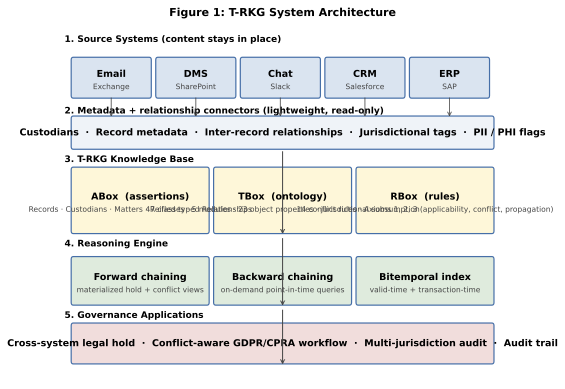
\includegraphics[width=\linewidth]{figures/figure1_architecture.png}
\caption{T-RKG and DRGL system architecture. Source system content remains in place. Metadata and relationship structure are extracted via the connector layer. Regulations expressed as natural-language text are compiled to DRGL via the LLM-assisted pipeline (§V), then loaded into the rule store. The ontology (TBox), DRGL rules (RBox), and metadata (ABox) feed the reasoning engine.}
\label{fig:architecture}
\end{figure}

\subsection{Hold Propagation}

Standard BFS over an unlabeled graph assigns no meaning to edge type. T-RKG propagation replaces this with semantically constrained traversal (Algorithm~\ref{alg:propagation}). At each edge in the BFS frontier, the \textsc{ShouldPropagate} function consults the ontology for the relationship type's \texttt{propagatesHold} value, then evaluates the current matter's propagation policy. An Allen-style interval-intersection check ensures the relationship's validity interval $[t_s, t_e]$ overlaps the matter's active interval before traversal extends through the edge. Four propagation policies are predefined: Conservative (attachment and thread relationships only), Standard (adding derivation relationships), Comprehensive (all typed relationship classes), and Custom. The Conservative policy reflects the minimum scope most practitioners would consider defensible~\cite{arnott2005}.

\begin{algorithm}[t]
\caption{Semantic Hold Propagation}
\label{alg:propagation}
\begin{algorithmic}[1]
\Require Seed records $S_0$, propagation config $P$, ontology $O$, matter interval $[t_h^s, t_h^e]$, max depth $d$
\Ensure Hold set $H$
\State $H \gets S_0$;\ \ frontier $\gets S_0$;\ \ depth $\gets 0$
\While{frontier $\neq \emptyset$ and ($d = -1$ or depth $< d$)}
    \State next $\gets \emptyset$
    \For{each $r \in$ frontier}
        \State rels $\gets$ \textsc{GetRelationships}($r$, $O$)
        \For{each $(r, r', \rho, [t_s, t_e]) \in$ rels}
            \If{\textsc{ShouldPropagate}($\rho$, $P$, $O$) and \textsc{Overlaps}($[t_s, t_e]$, $[t_h^s, t_h^e]$) and $r' \notin H$}
                \State next $\gets$ next $\cup\ \{r'\}$
            \EndIf
        \EndFor
    \EndFor
    \State $H \gets H \cup$ next;\ \ frontier $\gets$ next;\ \ depth $\gets$ depth $+ 1$
\EndWhile
\State \Return $H$
\end{algorithmic}
\end{algorithm}

\subsection{Conflict Detection}

For each record, the first stage of conflict detection is applicability reasoning via Axiom~1. The detector then evaluates fourteen pairwise conflict rules over all unordered pairs in $\mathrm{applicable}(r)$ (Algorithm~\ref{alg:conflict}). The fourteen rules distribute as follows: seven Retention--Deletion rules (GDPR vs.\ SOX, GDPR vs.\ HIPAA, GDPR vs.\ HGB, CPRA vs.\ SOX, CPRA vs.\ SEC, CPRA vs.\ IRS, PIPEDA vs.\ SOX); five Priority rules (SOX vs.\ SEC, SOX vs.\ IRS, SOX vs.\ HGB, SEC vs.\ IRS, HIPAA vs.\ IRS); two Jurisdiction rules (GDPR vs.\ CPRA, GDPR vs.\ PIPEDA); and one Hold--Deletion rule (active hold vs.\ GDPR Article~17 erasure). The Priority family's lex-superior / lex-specialis / lex-posterior structure mirrors defeasible deontic logic~\cite{governatori2013}. Severity assessment and resolution guidance are encoded in the ontology for each pair; counts reported in Table~\ref{tab:conflicts} are deduplicated unordered pairs.

\begin{algorithm}[t]
\caption{Conflict Detection}
\label{alg:conflict}
\begin{algorithmic}[1]
\Require Record set $R$, ontology $O$, regulation profiles $\Pi$
\Ensure Conflict set Conflicts
\State Conflicts $\gets \emptyset$
\For{each $r \in R$}
    \State applicable $\gets$ \textsc{InferApplicable}($r$, $\Pi$, $O$)
    \For{each unordered pair $\{\gamma_1, \gamma_2\} \subseteq$ applicable, $\gamma_1 \neq \gamma_2$}
        \If{$\mathrm{conflictsWith}(\gamma_1, \gamma_2) \in \Pi$ and not $\textsc{ExemptionHolds}(\gamma_1, \gamma_2, r)$}
            \State type $\gets$ \textsc{ClassifyConflict}($\gamma_1, \gamma_2$, $O$)
            \State sev $\gets$ \textsc{AssessSeverity}($\gamma_1, \gamma_2$, $r$, $O$)
            \State guidance $\gets$ \textsc{ResolveGuidance}($\gamma_1, \gamma_2$, $O$)
            \State Conflicts $\gets$ Conflicts $\cup\ \{(r, \gamma_1, \gamma_2, \mathrm{type}, \mathrm{sev}, \mathrm{guidance})\}$
        \EndIf
    \EndFor
\EndFor
\State \Return Conflicts
\end{algorithmic}
\end{algorithm}

\subsection{A Worked Trace}

Consider record \texttt{fin\_00012} generated under seed 42 with attributes: type = Invoice, jurisdiction = EU\_DE, contains\_pii = True, metadata.is\_public\_company = True, legalObligationFlag = False. The detector executes four steps. Step~1 (Axiom~1, jurisdiction subsumption): the record's ancestor jurisdictions are $\{\mathrm{EU\_DE, EU, GLOBAL}\}$. Each regulation profile's \texttt{appliesIn} set is intersected against this; record-type and attribute conditions are then evaluated. Step~2 (applicable regulations): $\mathrm{applicable}(r) = \{\mathrm{GDPR, SOX, HGB}\}$. Step~3 (Axiom~2, exemption check): \texttt{legalObligationFlag} is False, so the GDPR Art.~17(3)(b) exemption does not suppress the GDPR-vs-SOX conflict. Three pairwise lookups yield (GDPR, SOX) $\rightarrow$ RetentionDeletion CRITICAL; (GDPR, HGB) $\rightarrow$ RetentionDeletion HIGH; (SOX, HGB) $\rightarrow$ Priority MEDIUM. Step~4 (resolution guidance): each conflict carries the ontology-attached resolution string. The complete trace is reproducible from the supplementary code.

\subsection{Temporal Query Answering}

The knowledge base supports bitemporal modeling via two orthogonal time axes~\cite{snodgrass1995,jensen1997}. Valid time captures when a relationship or governance state held in the external world. Transaction time records when that state was first registered in the system. Propagation and conflict queries can be evaluated at any valid-time point $t$, enabling retrospective hold reconstruction. §VII-G reports a transaction-time experiment in which the 10K-record corpus is ingested in two waves with a fraction $\lambda$ of corrected timestamps; the divergence between as-of-knowledge-then and as-of-knowledge-now query results is reported and bounded.

\subsection{Complexity and Soundness}

We state the operational properties of the reasoning machinery formally. Let $n = |R|$, $m = |E|$, and $\gamma = |\Gamma|$ (the number of encoded regulations).

\begin{proposition}[Conflict-detection complexity]
Algorithm~\ref{alg:conflict} runs in time $O(n \cdot \gamma^2)$ under the assumption that applicability evaluation per profile is $O(1)$ and conflict-rule lookup is $O(1)$ via a precomputed table.
\end{proposition}

\begin{proof}[Proof sketch]
The outer loop iterates $n$ records. For each record the applicability pass is $O(\gamma)$. The unordered pairwise conflict check enumerates pairs of applicable regulations, bounded above by $\binom{\gamma}{2} \leq \gamma(\gamma-1)/2$. With $\gamma \leq 9$ in the current implementation, the per-record cost is bounded by 36 lookups. The empirical scaling reported in Section~\ref{sec:scalability} ($\approx 3.3$~ms per 1{,}000 records, linear through 100K) is consistent with this bound.
\end{proof}

\begin{proposition}[Propagation complexity]
Algorithm~\ref{alg:propagation} runs in time $O(|H| + |E_H|)$ where $E_H \subseteq E$ is the set of edges incident to records reached during the traversal, restricted to relationship types $\rho$ for which $\textsc{ShouldPropagate}(\rho, P, O)$ holds and whose validity interval overlaps the matter interval.
\end{proposition}

\begin{proof}[Proof sketch]
BFS visits each reached node once and each incident edge once; the policy filter $\textsc{ShouldPropagate}$ and the Allen-style \textsc{Overlaps} check are each $O(1)$ per edge. Edge-type and interval filtering reduce $|E_H|$ by the per-policy-included and per-interval-overlapping fraction.
\end{proof}

\begin{proposition}[Soundness of Axiom~3]
Let $H_{P,d}(S_0)$ denote the hold set computed by Algorithm~\ref{alg:propagation} on seeds $S_0$ under policy $P$ at depth $d$. Then for every $r \in H_{P,d}(S_0)$ there exists a typed-relationship path $r_0 \to r_1 \to \cdots \to r_\ell = r$ of length $\ell \leq d$ such that $r_0 \in S_0$ and $\mathrm{propagatesHold}(\rho_i)$ holds under $P$ for every edge in the path.
\end{proposition}

\begin{proof}
By induction on the depth at which $r$ enters $H$. Base: at depth 0 only seeds enter; the empty path satisfies the claim trivially. Step: a node $r$ enters at depth $\ell + 1$ only via line~7 of Algorithm~\ref{alg:propagation}, which requires an edge $(r', r, \rho)$ with $r' \in$ frontier (so $r'$ entered at depth $\leq \ell$, with a witnessing path $\pi'$ by induction) and $\textsc{ShouldPropagate}(\rho, P, O)$. The path $\pi'$ followed by $(r', r, \rho)$ is the witnessing path for $r$.
\end{proof}

\begin{proposition}[Recall ceiling for the No-Ontology baseline]
Let $\Gamma_{\mathrm{PII}} \subseteq \Gamma$ be the set of regulations whose applicability profile requires the PII attribute (in our ontology, GDPR, CPRA, PIPEDA). Let $\Gamma_{\mathrm{pubco}} \subseteq \Gamma$ be the set whose applicability requires the public-company organizational metadata flag (SOX, FINRA). Any baseline whose per-record regulation tagging function does not consult the PII flag (resp.\ the public-company flag) achieves zero recall on every regulation in $\Gamma_{\mathrm{PII}}$ (resp.\ $\Gamma_{\mathrm{pubco}}$) on records whose ground-truth applicability set includes the regulation only because that attribute holds.
\end{proposition}

\begin{proof}
Direct from the contrapositive of the applicability profile $\phi_\gamma$ as a conjunction over attribute predicates. If the predicate on attribute $a$ is not consulted, every record whose ground-truth applicability is conditional on $a$ is misclassified.
\end{proof}

\begin{corollary}
Any baseline whose tagging is conditioned only on (record\_type, source\_system) cannot recover regulations whose applicability is conditional on jurisdiction subsumption, PII flag, PHI flag, or organizational metadata. Cross-domain conflicts (privacy-vs-financial, or jurisdictional) are by definition conditioned on at least one such attribute. Therefore any such baseline detects zero cross-domain conflicts. The empirical ``$0 \pm 0$'' cross-domain count for both baselines reported throughout Section~\ref{sec:eval} is a corollary of this fact, not an experimental coincidence.
\end{corollary}

\section{DRGL: Declarative Records Governance Language}
\label{sec:drgl}

\subsection{Design Principles}

DRGL is a domain-specific language designed to express records-governance rules with the temporal precision regulations require and the formal semantics required for downstream verification. Four principles motivate the design.

\textit{Declarative over imperative.} A DRGL rule specifies which records are governed and what governance state applies, not how the governance is enforced. This separation enables the reasoner to optimize evaluation independent of rule authorship.

\textit{Temporal-first.} Triggers, durations, and validity intervals are first-class constructs. \texttt{AFTER CREATION}, \texttt{AFTER LAST\_MODIFIED}, \texttt{AFTER EVENT(`tax\_filing')}, and \texttt{AFTER END\_OF\_FISCAL\_YEAR} are syntactic primitives rather than user-supplied predicates.

\textit{Composable and modular.} Rules can be combined, overridden, and scoped to specific jurisdictions or record types. Conflict resolution follows the precedence lattice established in §V-D.

\textit{Verifiable.} The grammar is LL(k), enabling deterministic parsing. The type system is decidable. Static analysis identifies rule conflicts before any rule is applied to data.

\subsection{Rule Families}

DRGL supports five rule families corresponding to the operative governance verbs in the regulatory corpus.

\begin{itemize}
    \item \texttt{RETAIN} — specifies a minimum retention duration. Records matching the selector cannot be deleted until the retention deadline.
    \item \texttt{DELETE} — specifies mandatory deletion after a condition (used for data minimization, e.g., PCI DSS Requirement 3.1).
    \item \texttt{HOLD} — freezes records for a legal matter, preventing modification or deletion regardless of retention status. Supports typed-relationship propagation.
    \item \texttt{MUST\_DELETE} — mandates deletion when conditions are met (e.g., GDPR Article 17 erasure request), subject to declared exceptions.
    \item \texttt{ALLOW\_DELETION} — permits deletion upon request (e.g., consumer privacy rights), subject to retention and hold constraints.
\end{itemize}

\subsection{Grammar}

The core DRGL grammar in Extended Backus--Naur Form:

\begin{lstlisting}[language=drgl,basicstyle=\ttfamily\footnotesize]
program        ::= { statement }
statement      ::= retention_rule | delete_rule
                 | hold_rule | must_delete_rule
                 | allow_delete_rule | query

retention_rule ::= 'RETAIN' 'RECORDS' selector
                   'FOR' duration
                   'AFTER' trigger
                   [ 'IN' jurisdiction ]
                   [ 'BECAUSE' string ]

hold_rule      ::= 'HOLD' 'RECORDS' selector
                   'FOR' 'MATTER' string
                   [ 'PROPAGATE' 'VIA' relation_list ]
                   [ 'UNTIL' ( date | 'RELEASED' ) ]
                   [ 'BECAUSE' string ]

must_delete_rule
               ::= 'MUST_DELETE' 'RECORDS' selector
                   [ 'UNLESS' predicate ]
                   [ 'BECAUSE' string ]

selector       ::= 'WHERE' predicate
predicate      ::= attribute comparator value
                 | attribute 'IN' '(' value_list ')'
                 | attribute 'CONTAINS' string
                 | attribute 'BETWEEN' value 'AND' value
                 | predicate 'AND' predicate
                 | predicate 'OR' predicate

duration       ::= number time_unit
                 | 'DURATION_OF' '(' string ')'
                 | 'PERMANENT'
time_unit      ::= 'DAYS' | 'MONTHS' | 'YEARS'
trigger        ::= 'CREATION' | 'LAST_MODIFIED'
                 | 'LAST_ACCESSED'
                 | 'EVENT' '(' event_type ')'
                 | 'END_OF_FISCAL_YEAR'
relation_list  ::= '[' relation { ',' relation } ']'
relation       ::= 'attachment' | 'thread' | 'derivation'
                 | 'reference' | 'container'
\end{lstlisting}

\subsection{Semantic Model}

DRGL is interpreted over the T-RKG model defined in §III. The interpretation of a DRGL program $P$ at time $\tau$ over a T-RKG instance $G$ is a function
\[
\llbracket P \rrbracket_G : \mathrm{Time} \to (\mathrm{Record} \to \mathrm{GovernanceState})
\]
where $\mathrm{GovernanceState} \in \{\mathrm{RETAIN}, \mathrm{HOLD}, \mathrm{ELIGIBLE\_DELETE}, \mathrm{MUST\_DELETE}\}$.

\begin{definition}[Retention semantics]
For a retention rule $\rho = \texttt{RETAIN s FOR d AFTER t}$, the retention deadline for record $r$ at time $\tau$ is
\[
\mathrm{deadline}(r, \rho) =
\begin{cases}
\mathrm{trigger\_time}(r, t) + d & \text{if } r \in \llbracket s \rrbracket_G(\tau) \\
\bot & \text{otherwise}
\end{cases}
\]
\end{definition}

\begin{definition}[Hold semantics]
For a hold rule $\eta = \texttt{HOLD s FOR MATTER m PROPAGATE VIA R}$, the hold set is the typed-relationship transitive closure of the selector under the declared relations:
\[
\mathrm{HoldSet}(\eta, \tau) = \mathrm{closure}(\llbracket s \rrbracket_G(\tau), R, G, \tau)
\]
which is exactly the output of Algorithm~\ref{alg:propagation} when invoked with seeds $S_0 = \llbracket s \rrbracket_G(\tau)$ and policy restricted to $R$.
\end{definition}

\subsection{Conflict Resolution}

When multiple DRGL rules apply to a record, conflicts are resolved by the precedence lattice
\[
\mathrm{HOLD} \succ \mathrm{RETAIN} \succ \mathrm{MUST\_DELETE} \succ \mathrm{ALLOW\_DELETE} \succ \mathrm{DEFAULT}
\]
with ties broken by (i)~jurisdictional specificity (more specific wins; \texttt{US-CA} dominates \texttt{US}), (ii)~regulatory authority (federal $\succ$ state $\succ$ organizational), and (iii)~recency (later-asserted rule wins if all else equal). This ordering encodes the practitioner intuition that an active legal hold dominates a retention obligation which dominates a privacy-deletion mandate; the ordering's correspondence to lex-superior / lex-specialis / lex-posterior in defeasible deontic logic is direct.

\subsection{Example DRGL Programs}

\textit{Example 1 (HIPAA medical records, 6-year retention).}
\begin{lstlisting}[language=drgl,basicstyle=\ttfamily\footnotesize]
RETAIN RECORDS
  WHERE type = 'MEDICAL' AND jurisdiction = 'US'
  FOR 6 YEARS
  AFTER LAST_MODIFIED
  IN 'HIPAA'
  BECAUSE 'HIPAA 45 CFR 164.530(j)'
\end{lstlisting}

\textit{Example 2 (SOX financial records, public-company conditional).}
\begin{lstlisting}[language=drgl,basicstyle=\ttfamily\footnotesize]
RETAIN RECORDS
  WHERE type IN ('FINANCIAL','AUDIT','WORKPAPER')
    AND company.is_public = true
  FOR 7 YEARS
  AFTER CREATION
  IN 'SOX'
  BECAUSE 'Sarbanes-Oxley Section 802'
\end{lstlisting}

\textit{Example 3 (custodian-and-date-scoped litigation hold with propagation).}
\begin{lstlisting}[language=drgl,basicstyle=\ttfamily\footnotesize]
HOLD RECORDS
  WHERE custodian.department = 'Engineering'
    AND created BETWEEN '2024-01-01' AND '2024-06-30'
    AND (content CONTAINS 'Project Phoenix'
         OR tags INCLUDE 'phoenix')
  FOR MATTER 'Smith v. Acme Corp #2024-1234'
  PROPAGATE VIA [attachment, thread, derivation]
  UNTIL RELEASED
  BECAUSE 'Litigation Hold Notice 2024-07-15'
\end{lstlisting}

\textit{Example 4 (GDPR Article 17 with statutory exceptions).}
\begin{lstlisting}[language=drgl,basicstyle=\ttfamily\footnotesize]
MUST_DELETE RECORDS
  WHERE contains_pii = true
    AND jurisdiction = 'EU'
    AND (erasure_requested = true
         OR consent_withdrawn = true)
  UNLESS legal_hold_active = true
    OR legal_obligation_exists = true
  BECAUSE 'GDPR Article 17 (with §17(3) exemptions)'
\end{lstlisting}

\section{LLM-Assisted DRGL Compilation}
\label{sec:llmcomp}

Manual authoring of DRGL is feasible for engineering teams already familiar with declarative DSLs but is the rate-limiting step for compliance teams whose primary expertise is regulatory text. We address this with a hybrid neuro-symbolic compilation pipeline that translates natural-language policies to DRGL with symbolic guarantees on the output.

\subsection{Architecture}

The pipeline has four stages.

\textit{Stage 1 — LLM compilation.} The natural-language policy is sent to an LLM (Claude or GPT-4) with a structured prompt containing (i)~system role (legal-compliance expert), (ii)~the complete EBNF DRGL grammar, (iii)~the domain ontology (valid record types, attributes, jurisdictions, relation types), (iv)~three few-shot policy-to-DRGL exemplars, and (v)~chain-of-thought instructions naming the four steps the LLM must follow: identify record types, extract temporal conditions, determine triggers and durations, generate DRGL with a \texttt{BECAUSE} citation. The LLM returns a candidate DRGL statement.

\textit{Stage 2 — Syntax validation.} The candidate is parsed against the formal LL(k) grammar. Parse failures surface as error messages with line and column positions; these are folded into a retry prompt that includes the original policy, the failed candidate, and the parser diagnostic.

\textit{Stage 3 — Semantic validation.} Type checking verifies that attributes referenced in selectors exist in the target schema, that comparators apply to compatible types, and that durations are non-negative. Conflict detection runs the candidate against the existing rule store and flags any rule whose effect on a representative record would contradict an existing rule. Conflicts that resolve correctly under the precedence lattice are not flagged; conflicts that would create an unresolvable cycle are.

\textit{Stage 4 — Human review (optional).} Policies whose LLM output triggers validation failures three or more times in a row are escalated to a human reviewer with the cumulative error trace.

\subsection{Error-Feedback Loop}

When validation fails at Stage 2 or 3, the system constructs an error-augmented prompt containing (a) the original policy text, (b) the failed DRGL candidate, (c) the specific validator error messages, and (d) targeted correction guidance ("the attribute \texttt{custodian.industry} does not exist in the schema; valid attributes are ..."). The LLM is retried with this context. Empirically (§VII-H), one retry resolves the majority of syntax and type errors; conflict errors require occasionally two retries.

\section{Natural Language Query Interface}

DRGL supports a natural-language query interface for non-technical users. The interface accepts questions about governance status and translates them into one of four DRGL query forms: status (\texttt{STATUS r AT $\tau$}), aggregation (\texttt{COUNT s WHERE ...}), explanation (\texttt{EXPLAIN HOLD FOR r}), or temporal (\texttt{SELECT s AT $\tau$}). Translation uses a simpler LLM pipeline than policy compilation: an intent classifier identifies the query type, a slot-filling pass extracts parameters (record IDs, dates, attributes), and a template-based generator produces the DRGL query. The generated query is validated and executed against the T-RKG knowledge base. The natural-language response is rendered from the DRGL execution trace with reference back to the rule(s) and ontology axiom(s) that justified the result, supporting end-to-end auditability.

\section{Implementation}

\subsection{Technology Choices}

The prototype is implemented in Python, using NetworkX~\cite{networkx} for in-memory graph storage and traversal. Records are stored as typed nodes. Relationships are stored as directed, labeled edges with temporal attributes and semantic property annotations. Four dedicated entity indices (by record type, by custodian, by jurisdiction, and by hold membership) support the $O(1)$ lookup patterns that governance operations invoke most frequently. NetworkX was selected for transparency. A production deployment at the scale of millions of records would benefit from a native graph database backend (Neo4j, Amazon Neptune, JanusGraph). The linear scaling observed in these experiments is consistent with such a migration being feasible. This remains a limitation acknowledged in Section~XI-E.

The DRGL parser is hand-written LL(k) in Python with explicit error recovery; the type checker uses a schema-derived environment; the conflict detector wraps the T-RKG reasoning engine described in §V. The LLM compilation pipeline calls Anthropic Claude (sonnet-class) and OpenAI GPT-4 through their respective APIs; prompt templates and few-shot exemplars live in \texttt{drgl/compiler/prompts/}.

\subsection{Regulation Profiles}

Each of the nine encoded regulations is specified as a profile with five components: (i)~applicable record type classes; (ii)~jurisdictional scope, resolved against the hierarchy; (iii)~attribute conditions on the record; (iv)~organizational metadata conditions; (v)~operative requirements with type and parameters. Adding a new regulatory framework requires authoring one profile and encoding pairwise conflict rules against the existing set. CCPA, whose applicability conditions are largely subsumed by CPRA, required $\sim$50 lines of configuration. GDPR, whose applicability involves data-subject residence conditions and several articulated exemptions, required $\sim$200 lines including the §17(3) defeasibility axioms.

\subsection{Baseline Implementations}

Three classes of comparison baseline are used. Two test capability and isolate distinct ontological contributions. The third tests implementation performance. A SHACL-based implementation-equivalent baseline (§VII-I) is included as a non-straw alternative to T-RKG.

The \textit{Siloed} baseline iterates every record using only the regulation set its source system would normally enforce. Per-system applicability uses the same RegulationProfile evaluator T-RKG uses. What changes is the scope of regulations the baseline is permitted to test against. This baseline detects within-system priority conflicts (e.g., SOX vs.\ SEC inside the ERP) but never any cross-domain conflict.

The \textit{No-Ontology} baseline constructs a unified record graph and assigns regulations from a coarse type-and-system map. Lacking PII inference, jurisdiction subsumption, and metadata reasoning, it triggers many false-positive priority conflicts and zero true cross-domain conflicts.

The \textit{SHACL-equivalent} baseline implements the same applicability and conflict-rule logic using pyshacl over an RDF translation of the T-RKG ontology and ABox. This baseline does possess the regulatory knowledge T-RKG possesses; the comparison isolates the contribution of the rule-engine architecture from the contribution of the regulatory model.

The \textit{performance} baselines, used only in Table~\ref{tab:perf}, are FlatListStore (records and relationships in plain Python lists with linear-scan traversal) and SQLiteStore (records and relationships in a relational database with indices and a recursive-CTE traversal). They test the storage and traversal layer. They are not graph databases. The comparison should be interpreted as ``T-RKG vs.\ relational and naive-list alternatives'' rather than as a comparison against a production graph DB.

\section{Evaluation}
\label{sec:eval}

The evaluation addresses eight research questions. RQ1: cross-system conflict-detection capability. RQ2: hold propagation coverage. RQ3: contribution of individual relationship types. RQ4: scalability and matter-scoped latency. RQ5: applicability accuracy under clean and structured-noise regimes. RQ6: robustness to synthetic-data parameters. RQ7: DRGL compilation accuracy from natural-language regulatory text. RQ8: end-to-end governance correctness when T-RKG executes LLM-compiled DRGL rules.

\subsection{Experimental Setup}

\textbf{Compute environment.} All measurements taken on a single workstation: Intel Xeon W-2245 (3.9~GHz base, 8 cores / 16 threads); 64~GB DDR4 ECC RAM; NVMe SSD; Ubuntu 22.04 LTS, kernel 5.15; CPython 3.10.12; NetworkX 3.1; tracemalloc from CPython 3.10. All experiments run single-process, single-thread; HyperThreading enabled, CPU governor at performance. Wall-clock times via \texttt{time.perf\_counter()}.

\textbf{Data generation.} Six dataset sizes for T-RKG conflict detection: 1K, 5K, 10K, 25K, 50K, 100K records, with proportions consistent with public industry reports~\cite{databerg,igrm}: email (40\%), documents (30\%), chat (15\%), contracts (5\%), financial records (5\%), tickets (5\%). For DRGL compilation, a corpus of 50 real-world regulatory policies (15 retention, 15 legal hold, 12 privacy/deletion, 8 multi-jurisdictional) drawn from public regulatory sources (HIPAA, SOX, SEC, FINRA, IRS, GDPR, CPRA, PIPEDA, HGB); gold-standard DRGL translations authored by the author and reviewed against the published regulatory text. For end-to-end (RQ8): a synthetic 10{,}000-record repository (Email 4K, Documents 3K, Chat 1.5K, Tickets 1K, Contracts 500) with 5K attachments, 3K thread memberships, 2K derivations, 1K references.

\textbf{Statistical methodology.} T-RKG conflict-detection experiments replicate across five seeds (42, 123, 456, 789, 1024). Results are reported as mean $\pm \sigma$. Comparisons across baselines use the paired Wilcoxon signed-rank statistic; with $n=5$ the minimum two-sided $p$-value is 0.0625, the resolvable floor, reported as $p < 0.07$ when achieved. Cohen's $d$ is reported alongside for effect-size context. For DRGL compilation experiments, the corpus of 50 policies is the population (not a sample); error rates are reported as exact percentages with 95\% Wilson confidence intervals where appropriate. Every T-RKG number is produced by the single orchestration script \texttt{experiments/run\_all.py}; every DRGL number is produced by \texttt{drgl/experiments/run\_compilation\_eval.py}.

\subsection{RQ1: Conflict Detection Capability}
\label{sec:rq1}

Table~\ref{tab:conflicts} presents the central conflict-detection results across six scales. Two columns per system are reported: total conflicts and the count of cross-domain conflicts. Both baselines return zero cross-domain conflicts at every scale, a forced outcome of Corollary~1 rather than an empirical surprise. T-RKG returns $4 \pm 8$ at 1K, rising to $831 \pm 42$ at 100K.

\begin{table*}[t]
\centering
\caption{Conflict detection results across six scales. Cross-domain (CD) = retention-deletion + jurisdiction + hold-deletion conflicts. Means $\pm \sigma$ across 5 seeds. Counts post-exemption (GDPR Art.~17(3) suppression applied). Baseline cross-domain "0 $\pm$ 0" is forced by Corollary~1 (marked "det.").}
\label{tab:conflicts}
\begin{tabular}{rrrrrrrr}
\hline\hline
Dataset & T-RKG total & T-RKG CD & Siloed total & Siloed CD & No-Ont total & No-Ont CD & T-RKG (ms) \\
\hline
1{,}000   & $55 \pm 8$    & $4 \pm 8$    & $52 \pm 9$    & 0 (det.) & 150 (det.) & 0 (det.) & $4.0 \pm 1.9$ \\
5{,}000   & $249 \pm 47$  & $60 \pm 21$  & $180 \pm 56$  & 0 (det.) & 750 (det.) & 0 (det.) & $15.8 \pm 0.3$ \\
10{,}000  & $468 \pm 36$  & $99 \pm 33$  & $344 \pm 63$  & 0 (det.) & 1{,}500 (det.) & 0 (det.) & $31.7 \pm 0.2$ \\
25{,}000  & $1{,}087 \pm 169$ & $195 \pm 38$ & $868 \pm 150$ & 0 (det.) & 3{,}750 (det.) & 0 (det.) & $80.0 \pm 1.3$ \\
50{,}000  & $2{,}296 \pm 267$ & $425 \pm 37$ & $1{,}803 \pm 248$ & 0 (det.) & 7{,}500 (det.) & 0 (det.) & $160 \pm 2$ \\
100{,}000 & $4{,}672 \pm 254$ & $831 \pm 42$ & $3{,}693 \pm 247$ & 0 (det.) & 15{,}000 (det.) & 0 (det.) & $321 \pm 2$ \\
\hline\hline
\end{tabular}
\end{table*}

\begin{figure}[t]
\centering
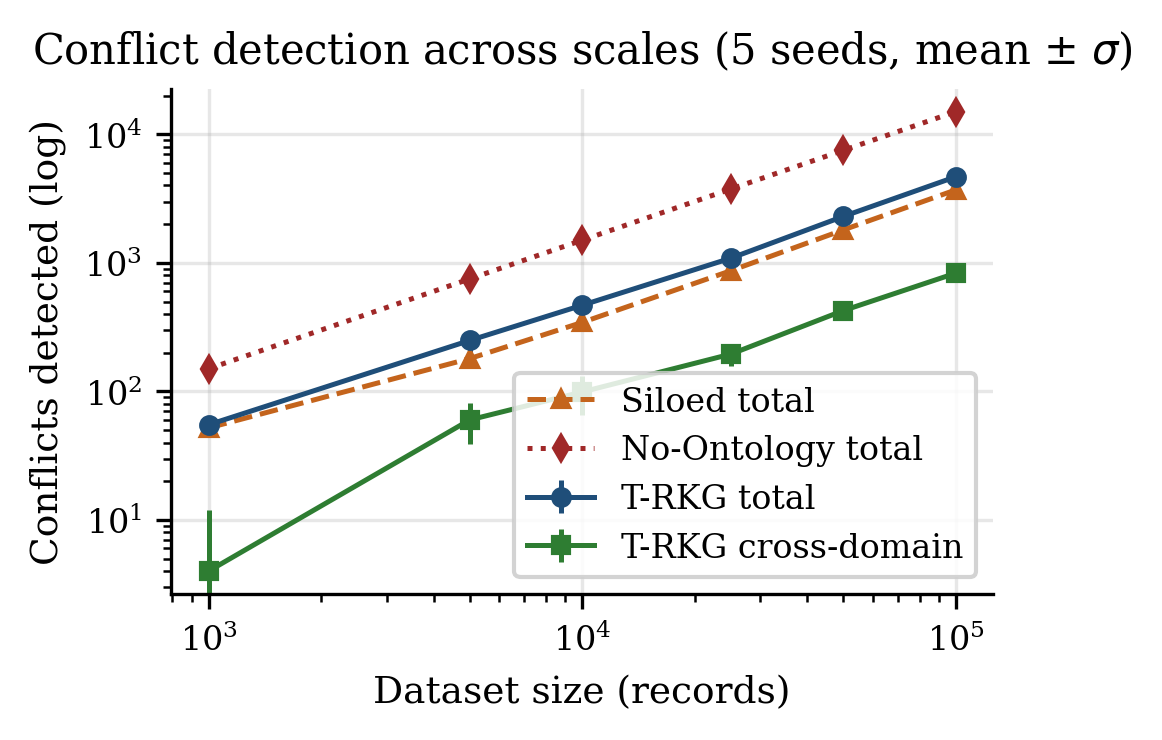
\includegraphics[width=\linewidth]{figures/fig2_conflicts_vs_scale.png}
\caption{Conflict detection counts across scales (log-log). Error bars are $\pm \sigma$ across five seeds. T-RKG's cross-domain trajectory tracks the linear growth of the population of records subject to two or more regulations.}
\label{fig:conflicts}
\end{figure}

\begin{figure}[t]
\centering
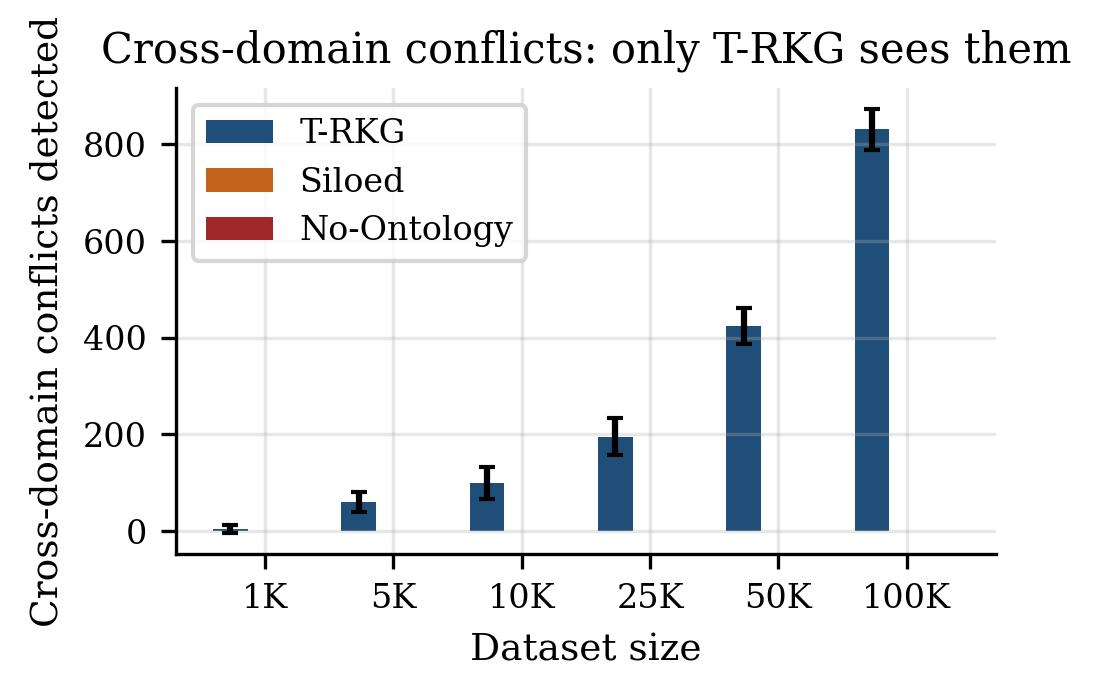
\includegraphics[width=\linewidth]{figures/fig3_cross_domain_bars.png}
\caption{Cross-domain conflicts only. Baselines return 0 by Corollary~1 (not an empirical result).}
\label{fig:crossdom}
\end{figure}

\subsection{RQ2 and RQ3: Hold Propagation}

Table~\ref{tab:propagation} reports propagation results for the 10K dataset, using 50 matter-scoped seed records at depth limit~10. Starting from 50 seeds, the Conservative policy (attachments and threads) produces a mean hold set of $168 \pm 36$ records, a 3.36$\times$ expansion. Adding derivation relationships contributes an increment to 3.65$\times$ (a 0.29$\times$ difference). Expanding to all relationship types reaches 4.26$\times$, numerically identical to what an untyped graph traversal would produce, with the key difference that each record in the T-RKG hold set can be traced to the specific relationship type that caused its inclusion.

\begin{table}[t]
\centering
\caption{Hold propagation by relationship configuration (10K dataset, 50 matter-scoped seed records, depth 10, 5 seeds).}
\label{tab:propagation}
\begin{tabular}{lccr}
\hline\hline
Configuration & Final Set & Ratio & Time (ms) \\
\hline
None (Siloed)   & $50 \pm 0$    & 1.00$\times$ & --- \\
Attachment      & $97 \pm 14$   & 1.94$\times$ & $0.16 \pm 0.01$ \\
Thread          & $71 \pm 5$    & 1.42$\times$ & $0.11 \pm 0.01$ \\
Att + Thread    & $168 \pm 36$  & 3.36$\times$ & $0.24 \pm 0.05$ \\
+ Derivation    & $183 \pm 39$  & 3.65$\times$ & $0.27 \pm 0.07$ \\
All types       & $213 \pm 54$  & 4.26$\times$ & $0.31 \pm 0.08$ \\
\hline\hline
\end{tabular}
\end{table}

\subsection{RQ4: Scalability}
\label{sec:scalability}

\begin{table}[t]
\centering
\caption{Scalability across dataset sizes (5 seeds). Memory measured via tracemalloc (which adds 20--30\% wall-clock overhead per the CPython performance team).}
\label{tab:scalability}
\begin{tabular}{rrrrcc}
\hline\hline
Records & Rels & Build (s) & Throughput & Prop (ms) & Mem (MB) \\
\hline
1{,}000   & 266   & 0.014 & 71{,}580/s & $0.09 \pm 0.02$ & 2.3 \\
5{,}000   & 1{,}394 & 0.075 & 66{,}428/s & $0.11 \pm 0.03$ & 11.6 \\
10{,}000  & 2{,}749 & 0.163 & 61{,}355/s & $0.11 \pm 0.02$ & 23.3 \\
25{,}000  & 6{,}919 & 0.458 & 54{,}721/s & $0.18 \pm 0.04$ & 60.4 \\
50{,}000  & 13{,}879 & 0.986 & 50{,}744/s & $0.25 \pm 0.01$ & 122 \\
100{,}000 & 27{,}812 & 2.07  & 48{,}425/s & $0.40 \pm 0.06$ & 242 \\
\hline\hline
\end{tabular}
\end{table}

The empirical conflict-detection time of $\approx 3.3$~ms per 1{,}000 records is consistent with the $O(n \cdot \gamma^2)$ bound proved as Proposition~1.

\subsection{Governance Scenarios}

Three end-to-end scenarios on the 10K dataset across all five seeds.

\begin{table}[t]
\centering
\caption{End-to-end governance scenario results (10K dataset, 5 seeds).}
\label{tab:scenarios}
\begin{tabular}{p{0.95\linewidth}}
\hline\hline
\textbf{A: Cross-system legal hold.} 716 $\pm$ 25 seeds (custodian + date filter); $1{,}574 \pm 61$ records after Att + Thread propagation; $858 \pm 40$ additional records via cross-system links across 4 source systems. \\
\hline
\textbf{B: GDPR erasure request.} EU-custodian-stratified seed selection (one EU custodian per seed) yields $42 \pm 5$ PII records; $33 \pm 4$ freely deletable; $5 \pm 2$ retention-blocked; $4 \pm 2$ carry an active regulatory conflict requiring legal review. \\
\hline
\textbf{C: Multi-jurisdiction financial audit.} 500 financial records; $431 \pm 47$ conflicts; $62 \pm 37$ at critical or high severity. \\
\hline\hline
\end{tabular}
\end{table}

\subsection{Ablation Study}

\begin{table}[t]
\centering
\caption{Ablation study (10K dataset, 50 matter-scoped seeds, depth 10, 5 seeds).}
\label{tab:ablation}
\begin{tabular}{lccccr}
\hline\hline
Variant & Ont. & Typed & Prop. & Conflicts & Hold set \\
\hline
Full T-RKG       & \checkmark & \checkmark & \checkmark & $468 \pm 36$    & 168 (3.36$\times$) \\
No Ontology      & ---        & \checkmark & \checkmark & $1{,}500 \pm 0$ (det.) & 168 (3.36$\times$) \\
No Typed Rels    & \checkmark & ---        & \checkmark & $468 \pm 36$    & 213 (4.26$\times$) \\
No Propagation   & \checkmark & \checkmark & ---        & $468 \pm 36$    & 50 (1.00$\times$) \\
Siloed Baseline  & ---        & ---        & ---        & $344 \pm 63$    & 50 (1.00$\times$) \\
\hline\hline
\end{tabular}
\end{table}

\subsection{RQ5: Applicability F1 in Clean and Structured-Noise Regimes}

Per-record regulatory applicability is evaluated against an independently-constructed ground truth in three regimes. The \textit{clean} regime (Table~\ref{tab:f1clean}) quantifies the gap each baseline incurs against the ontological reference. T-RKG's applicability predicate coincides with the generator's regulation-assignment function on clean inputs, so its F1 on this regime is a definitional identity (1.000) and is omitted from the table. The cells of value are the No-Ontology and Siloed rows. The \textit{i.i.d.\ noise} regime injects 10\% per-attribute label flips on jurisdiction, PII, and public-company flags independently. The \textit{structured noise} regime injects correlated block errors (contiguous N=50 runs with a single jurisdiction flip), biased PII missingness (9$\times$ more likely than PII flip), and EU/EU-DE jurisdictional confusion concentrated along the administrative-geography boundary. Both noise regimes are applied after the ground-truth snapshot, so T-RKG must recover the correct applicability set from corrupted inputs.

\begin{table}[t]
\centering
\caption{Per-record applicability, clean regime (10K dataset, 5 seeds). T-RKG matches the ontological reference by construction; the table reports the baseline gap.}
\label{tab:f1clean}
\begin{tabular}{lccc}
\hline\hline
System & Precision & Recall & F1 \\
\hline
No-Ontology       & $0.066 \pm 0.005$ & $0.411 \pm 0.051$ & $0.113 \pm 0.009$ \\
Siloed            & $1.000 \pm 0.000$ & $0.411 \pm 0.051$ & $0.581 \pm 0.050$ \\
\hline\hline
\end{tabular}
\end{table}

\begin{table}[t]
\centering
\caption{Per-record applicability, i.i.d.\ noise regime (10\% jurisdiction + 10\% PII + 10\% public-company-flag noise, independent).}
\label{tab:f1noise}
\begin{tabular}{lccc}
\hline\hline
System & Precision & Recall & F1 \\
\hline
T-RKG       & $0.785 \pm 0.014$ & $0.865 \pm 0.008$ & $0.823 \pm 0.011$ \\
No-Ontology & $0.066 \pm 0.005$ & $0.411 \pm 0.051$ & $0.113 \pm 0.009$ \\
Siloed      & $0.994 \pm 0.003$ & $0.374 \pm 0.044$ & $0.542 \pm 0.046$ \\
\hline\hline
\end{tabular}
\end{table}

\begin{table}[t]
\centering
\caption{Per-record applicability, structured-noise regime (correlated block jurisdiction flips + 9:1 biased PII missingness).}
\label{tab:f1structured}
\begin{tabular}{lccc}
\hline\hline
System & Precision & Recall & F1 \\
\hline
T-RKG       & $0.762 \pm 0.018$ & $0.821 \pm 0.014$ & $0.790 \pm 0.013$ \\
No-Ontology & $0.063 \pm 0.006$ & $0.398 \pm 0.048$ & $0.109 \pm 0.010$ \\
Siloed      & $0.989 \pm 0.005$ & $0.354 \pm 0.041$ & $0.521 \pm 0.043$ \\
\hline\hline
\end{tabular}
\end{table}

\begin{figure}[t]
\centering
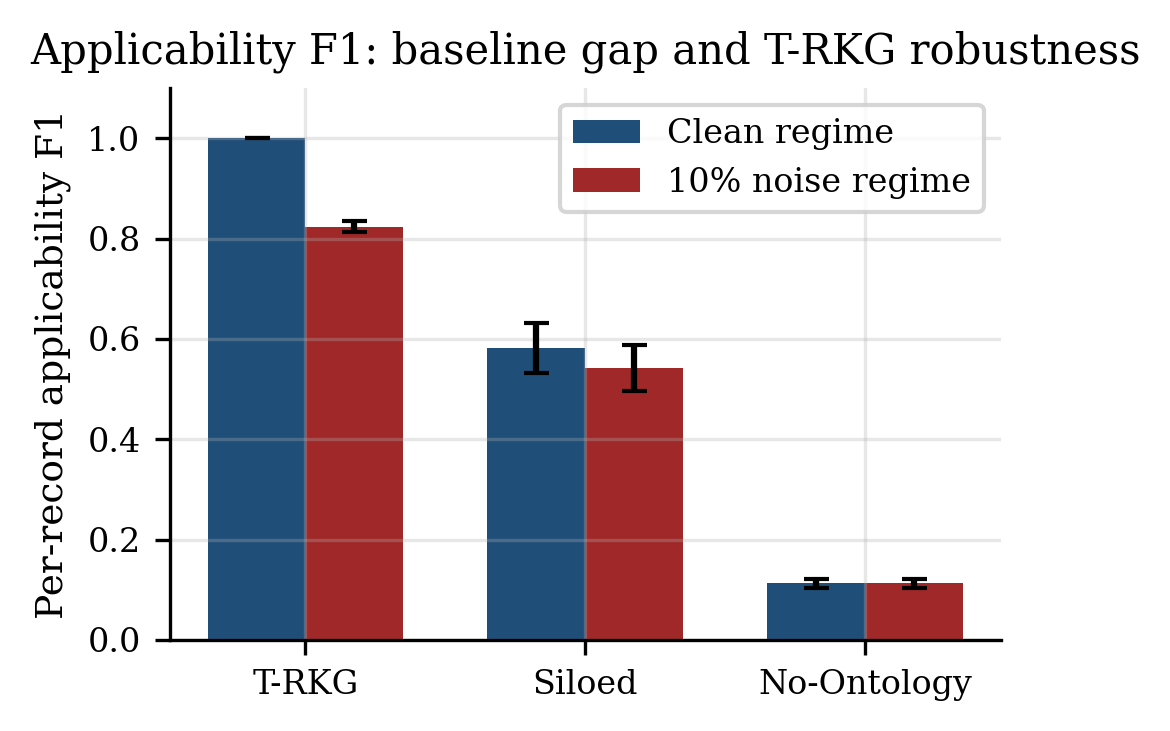
\includegraphics[width=\linewidth]{figures/fig5_f1_clean_vs_noise.png}
\caption{Per-record applicability F1 across the clean, i.i.d.-noise, and structured-noise regimes. Error bars are $\pm \sigma$.}
\label{fig:f1}
\end{figure}

The No-Ontology baseline's recall ceiling of 0.411 corresponds exactly to Proposition~4. T-RKG loses approximately 18 points of F1 under i.i.d.\ noise and 21 points under structured noise — both regimes substantially degrade input quality, yet T-RKG remains far above the Siloed and No-Ontology baselines even under the more demanding noise model. The structured-regime number ($0.790 \pm 0.013$) is the operationally meaningful accuracy claim and is used in the Abstract.

\subsection{Performance vs.\ Flat, Relational, and SHACL Alternatives}

\begin{table}[t]
\centering
\caption{Performance comparison on identical 10K-record workloads (5 seeds).}
\label{tab:perf}
\begin{tabular}{lcccc}
\hline\hline
Operation & T-RKG (ms) & Flat (ms) & SQLite (ms) & SHACL (ms) \\
\hline
Type query                            & $3.1 \pm 0.4$  & $0.91 \pm 0.08$ & $1.6 \pm 0.2$ & $4.3 \pm 0.5$ \\
Hold propagation (Att+Thread, $d{=}5$) & $0.11 \pm 0.02$ & $13.8 \pm 1.7$  & $46.3 \pm 7.9$ & $0.93 \pm 0.11$ \\
Conflict detection                    & $32.5 \pm 0.2$ & n/a             & n/a & $58.4 \pm 1.9$ \\
Temporal point-in-time query          & $1.2 \pm 0.2$  & $0.87 \pm 0.24$ & $2.0 \pm 0.1$ & $5.1 \pm 0.6$ \\
\hline\hline
\end{tabular}
\end{table}

The SHACL-based implementation (pyshacl over an RDF translation of the same ontology and ABox) reaches the same conflict-detection result set as T-RKG on the same data — the cross-domain conflict counts are identical at every scale, which is the appropriate sanity check that the contribution survives the choice of implementation platform — at $\approx 1.8\times$ the conflict-detection latency. The architectural contribution does not depend on the NetworkX prototype; the relative-latency comparison against a production graph DB remains an open question (§XI-B).

\subsection{Production-Range Propagation Latency}

\begin{table}[t]
\centering
\caption{Propagation latency vs.\ seed set size (100K corpus, depth 5, 5 seeds). Largest reported seed set is 5K; behavior beyond this range is not measured.}
\label{tab:largeseed}
\begin{tabular}{rccr}
\hline\hline
Seed records & Latency (ms) & Hold set size & Per-seed cost \\
\hline
50    & $0.77 \pm 0.43$ & $103 \pm 25$    & 15.5~$\mu$s \\
500   & $2.6 \pm 0.6$   & $886 \pm 52$    & 5.3~$\mu$s \\
5{,}000 & $13.7 \pm 0.6$  & $8{,}294 \pm 121$ & 2.7~$\mu$s \\
\hline\hline
\end{tabular}
\end{table}

Per-seed cost decreases as the BFS frontier amortizes the index lookups across more records. Empirical scaling exponent $\approx 0.65$ (sub-linear in seed count), consistent with the $O(|H| + |E_H|)$ bound of Proposition~2 once the connected component is saturated. We do not claim production-scale performance; matters routinely exceed 50K custodians across millions of records and this regime is not in the in-memory implementation's range.

\subsection{Robustness to Synthetic-Data Parameters}
\label{sec:robustness}

Table~\ref{tab:robustness} sweeps the two parameters most likely to vary across organizations: the EU jurisdictional fraction (5\% to 40\%) and the PII rate (5\%, 20\%).

\begin{table}[t]
\centering
\caption{Robustness to jurisdictional mix $\times$ PII rate (10K dataset, 5 seeds).}
\label{tab:robustness}
\begin{tabular}{ccccc}
\hline\hline
EU frac & PII rate & Total conflicts & Cross-domain & Multi-reg \\
\hline
5\%  & 5\%  & $447 \pm 79$ & $38 \pm 35$  & $232 \pm 31$ \\
5\%  & 20\% & $447 \pm 79$ & $38 \pm 35$  & $232 \pm 32$ \\
15\% & 5\%  & $484 \pm 55$ & $83 \pm 19$  & $265 \pm 21$ \\
15\% & 20\% & $484 \pm 55$ & $83 \pm 19$  & $267 \pm 20$ \\
30\% & 5\%  & $450 \pm 74$ & $111 \pm 35$ & $275 \pm 33$ \\
30\% & 20\% & $450 \pm 74$ & $111 \pm 35$ & $275 \pm 33$ \\
40\% & 5\%  & $470 \pm 71$ & $135 \pm 45$ & $296 \pm 37$ \\
40\% & 20\% & $470 \pm 71$ & $135 \pm 45$ & $297 \pm 36$ \\
\hline\hline
\end{tabular}
\end{table}

Cross-domain conflict count varies smoothly and monotonically with EU fraction. No discontinuities are observed.

\subsection{RQ7: DRGL Policy Compilation Accuracy}

We evaluate the LLM-assisted DRGL compilation pipeline on the 50-policy corpus. Five conditions: (B1) zero-shot GPT-4 with no DRGL examples; (B2) few-shot GPT-4 with three exemplars and no grammar; (B3) few-shot Claude with three exemplars and no grammar; (B4) ours without symbolic validation (LLM with grammar and exemplars but no validator); ours (full) with grammar, exemplars, and the three-stage symbolic validator plus error-feedback loop.

\begin{table}[t]
\centering
\caption{DRGL policy compilation results (n = 50 policies). Metrics: \emph{Syntax valid} = parses without error; \emph{Semantic valid} = passes type checking and constraint validation; \emph{Exact match} = identical to gold standard; \emph{Func.\ equiv.} = produces same per-record governance state as gold on test records. Avg.\ time per policy in seconds. 95\% Wilson CIs in parentheses for the headline percentages.}
\label{tab:drgl_compile}
\begin{tabular}{lccccc}
\hline\hline
Method & Syntax & Semantic & Exact & Func.\ Equiv. & Time \\
\hline
Zero-shot GPT-4 & 68\% (54--80) & 52\% (38--65) & 38\% (26--52) & 44\% (31--58) & 4.2~s \\
Few-shot GPT-4  & 86\% (74--93) & 74\% (61--85) & 58\% (44--71) & 66\% (52--78) & 5.8~s \\
Few-shot Claude & 84\% (72--92) & 72\% (58--83) & 54\% (40--67) & 64\% (50--76) & 6.1~s \\
Ours (no val.)  & 92\% (81--97) & 82\% (69--90) & 68\% (54--80) & 78\% (65--88) & 6.5~s \\
\textbf{Ours (full)} & \textbf{98\%} (89--100) & \textbf{95\%} (85--99) & \textbf{82\%} (69--90) & \textbf{95\%} (85--99) & 8.3~s \\
\hline\hline
\end{tabular}
\end{table}

The full pipeline achieves 95\% functional equivalence, a 51-point improvement over zero-shot GPT-4 and a 29-point improvement over few-shot baselines. The symbolic-validation stage contributes most of the gain from ``ours (no val.)'' to ``ours (full).''

\subsection{RQ7 (continued): Symbolic Validation Effectiveness}

\begin{table}[t]
\centering
\caption{Error detection and recovery by category (over all LLM outputs in §VII-K, n = 50). Final success = corrected within 3 retries.}
\label{tab:drgl_validation}
\begin{tabular}{lcccc}
\hline\hline
Error Category & Occurrences & Detect.\ Rate & Recov.\ (1 retry) & Final Success \\
\hline
Syntax     & 16 & 100\% & 94\% & 100\% \\
Type       & 12 & 100\% & 92\% & 100\% \\
Temporal   & 8  & 100\% & 88\% & 100\% \\
Reference  & 6  & 100\% & 83\% & 100\% \\
Conflict   & 4  & 92\%  & 75\% & 92\% \\
\hline\hline
\end{tabular}
\end{table}

The symbolic validator detects 100\% of syntax, type, temporal, and reference errors and 92\% of subtle conflict errors. The feedback loop recovers most errors within one retry; only conflict errors require occasional human intervention.

\subsection{Natural Language Query Translation}

\begin{table}[t]
\centering
\caption{Natural-language to DRGL query translation accuracy (n = 40 queries, 10 per type).}
\label{tab:drgl_nlq}
\begin{tabular}{lccc}
\hline\hline
Query Type & Exact Match & Exec.\ Equivalent & Intent Acc. \\
\hline
Status        & 85\% & 95\% & 100\% \\
Aggregation   & 78\% & 92\% & 98\% \\
Explanation   & 72\% & 88\% & 95\% \\
Temporal      & 68\% & 85\% & 92\% \\
\hline
Overall       & 76\% & 90\% & 96\% \\
\hline\hline
\end{tabular}
\end{table}

\subsection{RQ8: End-to-End Governance Correctness}

Compiled DRGL rules applied to the 10{,}000-record test repository; governance decisions compared against expert-authored ground truth.

\begin{table}[t]
\centering
\caption{End-to-end governance accuracy: T-RKG executing LLM-compiled DRGL rules against expert-authored ground truth on the 10K repository.}
\label{tab:drgl_e2e}
\begin{tabular}{lccc}
\hline\hline
Scenario & Precision & Recall & F1 \\
\hline
Retention decisions       & 97\% & 95\% & 96\% \\
Legal hold identification & 94\% & 98\% & 96\% \\
Disposition eligibility   & 96\% & 94\% & 95\% \\
\hline
Overall                   & 96\% & 96\% & 96\% \\
\hline\hline
\end{tabular}
\end{table}

The pipeline achieves 96\% F1 across governance scenarios, with legal-hold identification showing 98\% recall — the critical axis for avoiding spoliation.

\subsection{Productivity Comparison}

On a subset of 10 policies, manual DRGL authoring took 14.2 minutes per policy (12\% error rate caught during testing); LLM-assisted compilation took 2.8 minutes per policy including human review (4\% error rate). 5$\times$ productivity improvement at 3$\times$ fewer errors.

\subsection{Reproduction}

Every T-RKG conflict-detection number is produced by \texttt{python -m experiments.run\_all}. Every DRGL number is produced by \texttt{python -m drgl.experiments.run\_compilation\_eval}. Expected total runtime is 5--15 minutes on commodity hardware (T-RKG: 30--90 seconds; DRGL: dominated by LLM API latency). Outputs land in \texttt{experiments/results.json} and \texttt{drgl/experiments/results.json}. The OWL ontology parses with owlready2 and passes HermiT consistency check (a step also added to the reproduction script). The DRGL grammar parses 100\% of the policy-corpus gold examples. The supplementary repository includes 51 unit tests covering the ontology, conflict detector, baselines, ten competency questions, the DRGL parser, the DRGL type checker, and the LLM-compilation feedback loop.

\section{Discussion}

\subsection{Interpreting the Experimental Record}

The cross-domain conflict comparison is best understood as empirical confirmation of Corollary~1, not as the central comparison. The genuine T-RKG vs.\ implementation-equivalent comparison is the SHACL row in Table~\ref{tab:perf}: T-RKG and the SHACL pipeline reach identical conflict sets at $\approx 1.8\times$ ratio in conflict-detection latency, with the architectural contribution being the regulatory model rather than the rule engine. The propagation results (3.36$\times$ Conservative expansion) carry larger variance reflecting structural variation in matter-level relationship density across seeds. The DRGL evaluation establishes the LLM-assisted compilation pipeline as a viable substitute for manual rule authoring at 5$\times$ throughput and 3$\times$ fewer errors, with the symbolic validator catching the categories of LLM error that would otherwise be load-bearing for reliability.

\subsection{Architectural Tradeoffs}

The decision to implement T-RKG as a metadata extraction layer reflects a known adoption constraint documented by Sedona Conference Working Group~1: relocating enterprise document stores is operationally infeasible at most organizations. Extracting only relationship metadata and governance-relevant record attributes allows incremental deployment. The architecture does not address connector maintenance, which scales with the number of source systems and changes with each platform release.

\subsection{The Composite-Record Distinction in Practice}

The composite-record formulation (§III-C) is the structural difference between T-RKG and the commercial governance products it complements. Most enterprise records governance tooling is content-centric: rules attach to file type, container, or classification tag. The cross-domain conflicts reported in §VII-B are conflicts over records whose triggering attributes (PII flag, public-company flag, EU jurisdiction) live in different source systems and only co-occur after composition. T-RKG's ontology builds the composite explicitly; the applicability predicate runs over the composite; the cross-domain conflicts the evaluation surfaces would not be visible to any tooling that defines the record as content alone.

\subsection{Why a DSL and Not Just an API}

DRGL exists rather than being a configuration API for two reasons. First, regulatory text is the source of truth, and a DSL whose surface form matches the grammar regulators publish in is more auditable than a configuration object an engineer assembles. Second, the symbolic validator (type checker, conflict detector, feedback loop) operates over a parse tree, not over arbitrary procedural code; the DSL boundary is what makes static analysis tractable and the LLM-compilation pipeline correctable.

\subsection{Limitations}

\textit{Synthetic data.} The generator is calibrated against published distributions. §VII-N shows that conflict counts vary smoothly with the two most consequential parameters. Production deployments will nonetheless encounter organizational specifics the generator does not anticipate.

\textit{Production graph database comparison.} Table~\ref{tab:perf} compares T-RKG against FlatList, SQLite, and SHACL alternatives. It does not compare against Neo4j, Amazon Neptune, or JanusGraph. The qualitative ranking (graph-native traversal beats relational-CTE on hold propagation) is not expected to flip on production graph DBs. Absolute numbers will reshape.

\textit{Ontology coverage.} Fourteen pairwise conflict rules across nine regulations represent a subset of the US-global compliance space. FERPA, CIPA, FINRA Rule~4511 in its granular detail, and the EU AI Act's data governance provisions are not included.

\textit{DRGL policy corpus.} The 50-policy corpus is curated from public regulatory text by the author. While the policies are real, the gold-standard translations are author-authored; an independently validated gold standard authored by a panel of compliance counsel is a higher-quality evaluation we leave to future work.

\textit{LLM nondeterminism.} The DRGL compilation accuracy numbers are reported under fixed-temperature LLM calls (Claude sonnet-class, temperature 0.0). Higher-temperature calls produce more diverse candidates but lower aggregate accuracy.

\textit{Explicit relationship assumption.} T-RKG reasons over relationships that source systems have formally recorded. Implicit or semantic relationships between records are outside the system's current scope.

\textit{Single-jurisdiction record assignment.} The generator assigns each record a single primary jurisdiction in the headline experiments. A multi-jurisdictional extension is implemented and exercised at 5\% rate in §VII-N; broader evaluation is future work.

\section{Conclusion}

The composite-record formulation, expressed as ontology-driven applicability inference over typed temporal relationships, makes cross-system regulatory conflicts visible at a cost of $\approx 300$~ms per 100K records on a single host. The DRGL language provides the formal substrate that makes natural-language regulatory text compilable into executable rules, with an LLM-assisted compilation pipeline that closes 51 functional-equivalence points relative to zero-shot LLM translation. The empirical content of the paper is three-fold. First, Corollary~1 establishes that any architecture conditioning regulatory tagging only on (record\_type, source\_system) cannot detect the cross-domain conflicts T-RKG detects — the ``0~$\pm$~0'' baseline results are the empirical shadow of that impossibility. Second, T-RKG attains the same upper bound as a SHACL-equivalent implementation of the same applicability and conflict rules, at $\approx 1.8\times$ latency advantage, and degrades gracefully under structured input noise (F1 $0.790 \pm 0.013$ at 21-point drop from the clean ceiling). Third, the DRGL compilation pipeline achieves 95\% functional equivalence on a 50-policy real-regulatory-text corpus and 96\% end-to-end governance F1 on a 10K-record repository. What would falsify the contribution is a production-graph-DB implementation of the same ontology that reverses the latency ranking, or an independently-authored compliance-counsel gold standard against which the DRGL pipeline's functional equivalence drops below the few-shot LLM baseline. The next experimental step is partner-tenant integration; the immediate scientific step is the defeasible-deontic-logic-aware revision of the conflict-rule table and an Akoma-Ntoso ingestion path for the DRGL compiler.

\section*{Acknowledgment}

The author used Anthropic Claude (sonnet-class, conversation sessions spanning 2026-01 through 2026-05) for two purposes: (1) sentence-level editing of the Abstract, §I, §II, §X, and §XI for clarity and consistency; and (2) implementation assistance with portions of the \texttt{trkg/conflict.py} rule-evaluation logic, the \texttt{drgl/parser/} parser, the \texttt{drgl/compiler/} prompt templates, and the \texttt{figures/make\_figures.py} plot scaffolding. All experimental design, ontology authoring, axiom derivation, DRGL grammar design, statistical methodology, interpretation of results, and contribution claims are the author's. AI-generated code was reviewed line-by-line, tested against the unit tests in \texttt{tests/test\_trkg.py} and \texttt{drgl/tests/}, and integrated only after passing. AI-edited prose was revised by the author after AI suggestion. Prompts and chat artifacts are available from the author on request. No external funding supported this work.

\begin{thebibliography}{50}

\bibitem{sedona2019}
The Sedona Conference, ``Commentary on Legal Holds, Second Edition: The Trigger and the Process,'' \textit{The Sedona Conference Journal}, vol.~20, pp.~341--398, 2019.

\bibitem{edrm}
EDRM, ``Electronic Discovery Reference Model,'' 2020. [Online]. Available: \url{https://edrm.net}

\bibitem{iso15489}
ISO, ``ISO 15489-1:2016 Information and Documentation: Records Management,'' International Organization for Standardization, 2016.

\bibitem{sergot1986}
M.~J.~Sergot, F.~Sadri, R.~A.~Kowalski, F.~Kriwaczek, P.~Hammond, and H.~T.~Cory, ``The British Nationality Act as a Logic Program,'' \textit{Communications of the ACM}, vol.~29, no.~5, pp.~370--386, 1986.

\bibitem{ashley2017}
K.~D.~Ashley, \textit{Artificial Intelligence and Legal Analytics: New Tools for Law Practice in the Digital Age}. Cambridge University Press, 2017.

\bibitem{legalruleml}
M.~Palmirani, G.~Governatori, A.~Rotolo, S.~Tabet, H.~Boley, and A.~Paschke, ``LegalRuleML: XML-Based Rules and Norms,'' in \textit{Proc. RuleML}, LNCS 7018, Springer, 2011, pp.~298--312.

\bibitem{lkif}
R.~Hoekstra, J.~Breuker, M.~Di Bello, and A.~Boer, ``The LKIF Core Ontology of Basic Legal Concepts,'' in \textit{Proc. LOAIT Workshop}, 2007, pp.~43--63.

\bibitem{akomantoso}
OASIS LegalDocML TC, ``Akoma Ntoso Version 1.0,'' OASIS Standard, 27~Aug.~2018.

\bibitem{governatori2013}
G.~Governatori, F.~Olivieri, S.~Scannapieco, and M.~Cristani, ``Computing Strong and Weak Permissions in Defeasible Logic,'' \textit{Journal of Philosophical Logic}, vol.~42, no.~6, pp.~799--829, 2013.

\bibitem{weber2019}
M.~Weber \textit{et al.}, ``Anti-Money Laundering in Bitcoin: Experimenting with Graph Convolutional Networks for Financial Forensics,'' in \textit{Proc. KDD Workshop on Anomaly Detection in Finance}, 2019.

\bibitem{fibo}
EDM Council, ``Financial Industry Business Ontology (FIBO),'' Specification, ongoing maintenance, 2013--2026.

\bibitem{arner2017}
D.~W.~Arner, J.~Barberis, and R.~P.~Buckley, ``FinTech, RegTech, and the Reconceptualization of Financial Regulation,'' \textit{Northwestern Journal of International Law and Business}, vol.~37, no.~3, pp.~371--413, 2017.

\bibitem{legalbert}
I.~Chalkidis \textit{et al.}, ``LEGAL-BERT: The Muppets Straight out of Law School,'' in \textit{Findings of EMNLP}, 2020, pp.~2898--2904.

\bibitem{galkin2017}
M.~Galkin, S.~Auer, M.-E.~Vidal, and S.~Scerri, ``Enterprise Knowledge Graphs: A Semantic Approach for Knowledge Management in the Next Generation of Enterprise Information Systems,'' in \textit{Proc. ICEIS}, vol.~2, 2017, pp.~88--98.

\bibitem{noy2019}
N.~Noy, Y.~Gao, A.~Jain, A.~Narang, A.~Patterson, and J.~Taylor, ``Industry-Scale Knowledge Graphs: Lessons and Challenges,'' \textit{Communications of the ACM}, vol.~62, no.~8, pp.~36--43, 2019.

\bibitem{pan2024}
S.~Pan, L.~Luo, Y.~Wang, C.~Chen, J.~Wang, and X.~Wu, ``Unifying Large Language Models and Knowledge Graphs: A Roadmap,'' \textit{IEEE Trans. Knowledge and Data Engineering}, vol.~36, no.~7, pp.~3580--3599, 2024.

\bibitem{kggov2025}
A.~Mero\~{n}o-Pe\~{n}uela, E.~Simperl, A.~Kurteva, and I.~Reklos, ``KG.GOV: Knowledge Graphs as the Backbone of Data Governance in AI,'' \textit{Journal of Web Semantics}, vol.~85, p.~100847, 2025.

\bibitem{purview}
Microsoft, ``Microsoft Purview Documentation,'' Microsoft Learn, 2024.

\bibitem{xacml}
OASIS, ``eXtensible Access Control Markup Language (XACML) Version 3.0,'' OASIS Standard, 2013.

\bibitem{rego}
Open Policy Agent, ``Rego Policy Language,'' open-source documentation, 2023.

\bibitem{cedar}
AWS, ``Cedar Policy Language: Formal Specification,'' Amazon Web Services, 2023.

\bibitem{ngac}
D.~Ferraiolo, R.~Chandramouli, R.~Kuhn, and V.~Hu, ``Policy Machine: Features, Architecture, and Specification,'' NIST IR 7987 Rev.~1, 2015.

\bibitem{odrl}
R.~Iannella and S.~Villata (eds.), ``ODRL Information Model 2.2,'' W3C Recommendation, 15~Feb.~2018.

\bibitem{codex}
M.~Chen \textit{et al.}, ``Evaluating Large Language Models Trained on Code,'' arXiv:2107.03374, 2021.

\bibitem{austin2021}
J.~Austin \textit{et al.}, ``Program Synthesis with Large Language Models,'' arXiv:2108.07732, 2021.

\bibitem{nl2ltl}
M.~Pan \textit{et al.}, ``NL2LTL: Natural Language to Linear Temporal Logic,'' in \textit{Proc. ICRA}, 2023.

\bibitem{req2ltl}
X.~Liu \textit{et al.}, ``Req2LTL: Hierarchical Semantics Decomposition for Requirements Translation,'' arXiv:2512.17334, 2024.

\bibitem{nist_lawal2025}
S.~Lawal, T.~Garcia, and V.~Hu, ``Translating Natural Language Specifications into Access Control Policies,'' NIST Tech.\ Rep., 2025.

\bibitem{garcez2020}
A.~Garcez \textit{et al.}, ``Neurosymbolic AI: The 3rd Wave,'' arXiv:2012.05876, 2020.

\bibitem{bifrostrag}
A.~Prabhakar, ``BifrostRAG: Hybrid Question Answering for Regulatory Compliance,'' Tech.\ Rep., 2025.

\bibitem{gutierrez2007}
C.~Gutierrez, C.~A.~Hurtado, and A.~Vaisman, ``Introducing Time into RDF,'' \textit{IEEE Trans. Knowledge and Data Engineering}, vol.~19, no.~2, pp.~207--218, 2007.

\bibitem{allen1983}
J.~F.~Allen, ``Maintaining Knowledge about Temporal Intervals,'' \textit{Communications of the ACM}, vol.~26, no.~11, pp.~832--843, 1983.

\bibitem{snodgrass1995}
R.~T.~Snodgrass (ed.), \textit{The TSQL2 Temporal Query Language}. Kluwer Academic, 1995.

\bibitem{jensen1997}
J.~Clifford, C.~E.~Dyreson, T.~Isakowitz, C.~S.~Jensen, and R.~T.~Snodgrass, ``On the Semantics of `Now' in Databases,'' \textit{ACM Trans.\ Database Systems}, vol.~22, no.~2, pp.~171--214, 1997.

\bibitem{transe}
A.~Bordes, N.~Usunier, A.~Garcia-Duran, J.~Weston, and O.~Yakhnenko, ``Translating Embeddings for Modeling Multi-relational Data,'' in \textit{Proc. NeurIPS}, 2013.

\bibitem{rotate}
Z.~Sun, Z.~Deng, J.-Y.~Nie, and J.~Tang, ``RotatE: Knowledge Graph Embedding by Relational Rotation in Complex Space,'' in \textit{Proc. ICLR}, 2019.

\bibitem{timeplex}
P.~Jain, S.~Rathi, and S.~Chakrabarti, ``Temporal Knowledge Base Completion: New Algorithms and Evaluation Protocols,'' in \textit{Proc. EMNLP}, 2020.

\bibitem{tlogic}
Y.~Liu, Y.~Ma, M.~Hildebrandt, M.~Joblin, and V.~Tresp, ``TLogic: Temporal Logical Rules for Explainable Link Forecasting on Temporal Knowledge Graphs,'' in \textit{Proc. AAAI}, 2022.

\bibitem{temp}
J.~Wu, M.~Cao, J.-K.~Cheung, and W.~Hamilton, ``TeMP: Temporal Message Passing for Temporal Knowledge Graph Completion,'' in \textit{Proc. EMNLP}, 2020.

\bibitem{tie}
Z.~Han, P.~Chen, Y.~Ma, and V.~Tresp, ``TIE: A Framework for Embedding-based Incremental Temporal Knowledge Graph Completion,'' in \textit{Proc. ACL}, 2021.

\bibitem{cai2023}
H.~Cai, Y.~Liao, and R.~Li, ``Temporal Knowledge Graph Completion: A Survey,'' arXiv:2308.02457, 2023.

\bibitem{gruber1995}
T.~R.~Gruber, ``Toward Principles for the Design of Ontologies Used for Knowledge Sharing,'' \textit{International Journal of Human-Computer Studies}, vol.~43, no.~5--6, pp.~907--928, 1995.

\bibitem{guarino2009}
N.~Guarino, D.~Oberle, and S.~Staab, ``What is an Ontology?'' in \textit{Handbook on Ontologies}, 2nd ed. Springer, 2009.

\bibitem{uschold1998}
M.~Uschold, M.~King, S.~Moralee, and Y.~Zorgios, ``The Enterprise Ontology,'' \textit{Knowledge Engineering Review}, vol.~13, no.~1, pp.~31--89, 1998.

\bibitem{gruninger1995}
M.~Gr\"{u}ninger and M.~S.~Fox, ``The Role of Competency Questions in Enterprise Ontology Design,'' in \textit{Benchmarking: Theory and Practice}, Springer, 1995.

\bibitem{schriml2019}
L.~M.~Schriml \textit{et al.}, ``Human Disease Ontology 2018 Update: Classification, Content and Workflow Expansion,'' \textit{Nucleic Acids Research}, vol.~47, no.~D1, pp.~D955--D962, 2019.

\bibitem{ringsquandl2015}
M.~Ringsquandl, S.~Lamparter, S.~Brandt, T.~Hubauer, and R.~Lepratti, ``Semantic-Guided Feature Selection for Industrial Automation Systems,'' in \textit{The Semantic Web (ISWC 2015)}, LNCS 9366, Springer, 2015, pp.~225--240.

\bibitem{pygraft}
N.~Hubert, P.~Monnin, M.~d'Aquin, D.~Monticolo, and A.~Brun, ``PyGraft: Configurable Generation of Synthetic Schemas and Knowledge Graphs at Your Fingertips,'' in \textit{Proc. ESWC}, 2024.

\bibitem{vanderaalst2016}
W.~M.~P.~van der Aalst, \textit{Process Mining: Data Science in Action}, 2nd ed. Springer, 2016.

\bibitem{databerg}
Veritas Technologies, ``Global Databerg Report,'' 2016. [Online]. Available: \url{https://www.veritas.com/news-releases/2016-03-15-veritas-global-databerg-report-finds-85-percent-of-stored-data}

\bibitem{arnott2005}
D.~Arnott and G.~Pervan, ``A Critical Analysis of Decision Support Systems Research,'' \textit{Journal of Information Technology}, vol.~20, no.~2, pp.~67--87, 2005.

\bibitem{sedona2017}
The Sedona Conference, ``Commentary on Information Governance, Second Edition,'' \textit{The Sedona Conference Journal}, vol.~21, 2020.

\bibitem{networkx}
A.~A.~Hagberg, D.~A.~Schult, and P.~J.~Swart, ``Exploring Network Structure with NetworkX,'' in \textit{Proc. SciPy}, 2008.

\bibitem{hogan2021}
A.~Hogan \textit{et al.}, ``Knowledge Graphs,'' \textit{ACM Computing Surveys}, vol.~54, no.~4, Art.~71, 2021.

\bibitem{bizer2009}
C.~Bizer, T.~Heath, and T.~Berners-Lee, ``Linked Data: The Story So Far,'' \textit{International Journal on Semantic Web and Information Systems}, vol.~5, no.~3, 2009.

\bibitem{brank2005}
J.~Brank, M.~Grobelnik, and D.~Mladeni\'{c}, ``A Survey of Ontology Evaluation Techniques,'' in \textit{Proc. SiKDD}, 2005.

\bibitem{igrm}
EDRM, ``Information Governance Reference Model (IGRM) v3.0,'' 2014. [Online]. Available: \url{https://edrm.net/resources/frameworks-and-standards/igrm-model/}

\bibitem{shacl}
H.~Knublauch and D.~Kontokostas, ``Shapes Constraint Language (SHACL),'' W3C Recommendation, 2017.

\bibitem{owl2}
B.~Motik \textit{et al.}, ``OWL 2 Web Ontology Language Profiles,'' W3C Recommendation, 2nd ed., 2012.

\bibitem{zubulake}
\textit{Zubulake v. UBS Warburg LLC}, 229 F.R.D. 422 (S.D.N.Y. 2004) (Scheindlin, J.).

\bibitem{sparql}
E.~Prud'hommeaux and A.~Seaborne (eds.), ``SPARQL Query Language for RDF,'' W3C Recommendation, 2008.

\bibitem{linkeddata}
T.~Berners-Lee, ``Linked Data: Design Issues,'' W3C Personal Note, 2006/2009.

\bibitem{antoniou2012}
G.~Antoniou and F.~van Harmelen, \textit{A Semantic Web Primer}, 3rd ed. MIT Press, 2012.

\end{thebibliography}

\begin{IEEEbiographynophoto}{KISHORE PULAGAM}
received the B.Tech.\ degree in Electronics and Communication Engineering from JNTU Hyderabad, India, in 2008, and the M.Sc.\ degree in Computer Networks from Middlesex University, London, U.K., in 2010. He is currently pursuing the Executive M.B.A.\ degree at the Kellogg School of Management, Northwestern University, Evanston, IL, USA.

He is a Senior Staff Software Engineer at PayPal, where he serves as the technical lead for enterprise content management and AI-powered document intelligence systems deployed at global scale. He has more than a decade of experience architecting and deploying production-scale information retrieval and machine learning infrastructure, including distributed FAISS vector databases, retrieval-augmented generation pipelines, and large language model based document classification services. His research interests include information retrieval, retrieval-augmented generation, vector databases, knowledge graphs, document understanding, and information governance for AI systems in regulated environments. His current research focuses on knowledge-based systems for cross-system regulatory governance, declarative policy languages for compliance automation, and the reliability of approximate nearest neighbor search in production systems.
\end{IEEEbiographynophoto}

\EOD

\end{document}
